%%
%% MLSALT project dissertation template.
%%
%% Currently designed for printing two-sided, but if you prefer to
%% print single-sided just remove ",twoside,openright" from the
%% \documentclass[] line below.
%%
%%
%%   FTL, July 2016
%%   SMH, May 2010.


\documentclass[a4paper,12pt,twoside,openright]{report}

\usepackage{xcolor}
\usepackage{amsfonts}

\usepackage{hhtensor}
\usepackage{mathtools}

\newcommand{\RR}{\mathbb{R}}
\newcommand{\NN}{\mathbb{N}}
\newcommand{\m}{\vec{m}}
\newcommand{\s}{\vec{s}}
\renewcommand{\o}{\vec{o}}
\newcommand{\x}{\vec{x}}
\newcommand{\y}{\vec{y}}
\newcommand{\U}{\matr{U}}
\newcommand{\V}{\matr{V}}
\newcommand{\W}{\matr{W}}
\DeclareMathOperator*{\softmax}{softmax}

\newcommand{\todo}[1]{}
\renewcommand{\todo}[1]{{\color{red} TODO\@: {#1}}}


%%
%% EDIT THE BELOW TO CUSTOMIZE
%%

\def\authorname{Feynman T. Liang\xspace}
\def\authorcollege{Churchill College\xspace}
\def\authoremail{fl350@cam.ac.uk}
\def\dissertationtitle{BachBot: Sequence Modeling of Bach Chorales}
\def\wordcount{\todo{DO THIS}}

\usepackage{epsfig,graphicx,parskip,setspace,tabularx,xspace}
\usepackage{hyperref}

\usepackage[acronym,xindy]{glossaries}
\makeglossaries
\usepackage[xindy]{imakeidx}
\makeindex
\loadglsentries[main]{glossary}

%% START OF DOCUMENT
\begin{document}


%% FRONTMATTER (TITLE PAGE, DECLARATION, ABSTRACT, ETC)
\pagenumbering{gobble}
\pagestyle{empty}
\singlespacing
% title page information
\begin{titlepage}

\begin{center}
\noindent
\huge
\dissertationtitle \\
\vspace*{\stretch{1}}
\end{center}

\begin{center}
\noindent
\huge
\authorname \\
\Large
\authorcollege      \\[24pt]

\includegraphics{CUni3.eps}
\end{center}

\vspace{24pt}

\begin{center}
\noindent
\large
{\it A dissertation submitted to the University of Cambridge \\
in partial fulfilment of the requirements for the degree of \\
Master of Philosophy in Machine Learning, Speech, and Language Technology}
\vspace*{\stretch{1}}
\end{center}

\begin{center}
\noindent
University of Cambridge \\
Engineering Department \\
Trumpington Steet \\
Cambridge CB2 1PZ       \\
{\sc United Kingdom}    \\
\end{center}

\begin{center}
\noindent
Email: \authoremail \\
\end{center}

\begin{center}
\noindent
\today
\end{center}

\end{titlepage}

\newpage
\vspace*{\fill}

\onehalfspacing
\documentclass[dissertation.tex]{subfiles}
\begin{document}
\newpage
{\Huge \bf Declaration}

\vspace{24pt}

I \authorname of \authorcollege, being a candidate for the M.Phil in Machine
Learning, Speech, and Language Technology, hereby declare that this report and
the work described in it are my own work, unaided except as may be specified
below, and that the report does not contain material that has already been used
to any substantial extent for a comparable purpose.

\vspace{24pt}
Total word count: \wordcount

\vspace{60pt}
\textbf{Signed}:

\vspace{12pt}
\textbf{Date}:


\vfill

This dissertation is copyright \copyright 2016 \authorname.
\\
All trademarks used in this dissertation are hereby acknowledged.



\newpage
\vspace*{\fill}
\end{document}

\singlespacing
\newpage
{\Huge \bf Abstract}
\vspace{24pt} 


This is the abstract. Write a summary of the whole thing. Make 
sure it fits in one page. 


\newpage
\vspace*{\fill}


\pagenumbering{roman}
\setcounter{page}{0}
\pagestyle{plain}
\tableofcontents
\printglossary[title=List of Abbreviations and Symbols]
\listoffigures
\listoftables

\onehalfspacing

%% START OF MAIN TEXT

\pagenumbering{arabic}
\setcounter{page}{1}

\documentclass[dissertation.tex]{subfiles}
\begin{document}

\chapter{Introduction}

% This is the introduction where you should introduce your work.  In
% general the thing to aim for here is to describe a little bit of the
% context for your work --- why did you do it (motivation), what was the
% hoped-for outcome (aims) --- as well as trying to give a brief
% overview of what you actually did.

% It's often useful to bring forward some ``highlights'' into
% this chapter (e.g.\ some particularly compelling results, or
% a particularly interesting finding).

% It's also traditional to give an outline of the rest of the
% document, although without care this can appear formulaic
% and tedious. Your call.

\begin{quote}
  What can we say about the perception of music by the silent majority of
  listeners, those for whom music is written but who neither create music nor
  can articulate their musical experience? How do they acquire their
  demonstrably sophisticated intuitions about music patterns
  typical of their culture? Experiments in the cognitive psychology of music
  have cast some light on the first question. Recent developments in neural net learning
  now enables us to explore the second.
\end{quote}\cite{bharucha1989modeling}

Bringing together ideas from language modelling, deep learning, and music
psychology, we develop a generative model for music and conduct a large-scale
subjective evaluation. Our results validate our success: participants were only
5\% more likely to identify an original Bach composition from a sample from
BachBot. To our knowledge, no prior work in automatic composition has carried
out a study at this scale.

Our fundamental question is this: have advances in deep learning enabled
construction of musical models capable of deceiving human listeners. To answer this
question, we build a model incorporating the current state-of-the-art in deep
neural sequence modelling and conduct a large-scale musical Turing test. Our
results suggest an undeniable yes.

Our contributions incude:
\begin{enumerate}
    \item A note-by-note sequential representation for polyphonic music amenable to processing with
        standard sequence models
    \item A rigorous investigation of how recent deep learning advances
      (dropout\cite{srivastava2014dropout}, batch
      normalization\cite{ioffe2015batch}, RNN architectures) can be applied to
      improve probabilistic modelling of music data
    \item A connectionist model for Bach chorales which avoids domain-specific
      feature engineering and is capable of composing, completing, harmonizing,
      and scoring polyphonic scores
    \item The first large-scale music Turing test with over \todo{XXX} participants
\end{enumerate}


While deep learning has revolutionized computer vision and natural language
processing, its applications to other domains are still emerging. This
dissertation is concerned with the applications of deep learning to a new
problem domain: music scores.

In this work, we investigate how sequence probability models parameterized by
deep recurrent neural networks can be used as generative models over scores of
music. Such a model has a variety of applications within computational music
theory. The aim of this work is to investigate applications on two particular
tasks: melody harmonization and automatic composition.

Every aspiring music theorist is at some point tasked with composing simple
pieces of music in order demonstrate understanding of the harmonic rules of
Western classical music. These pedagogical exercises often include
harmonization of chorale melodies, a task which is viewed as sufficiently
constrained to allow a composer's skill to be judged. A generative model
for music scores can be applied to this task by conditioning on the melody
line and sampling the conditional distribution for possible harmonizations.

A more difficult task is automatic composition, where the composer is tasked
with producing an original composition of a particular musical style. The open
nature of this task enables a composer to simultaneously demonstrate their
creativity along with understanding of music theory. However, this lack of
constraints and loose definition of musical style makes it more difficult to
evaluate the quality of the output. To apply a generative model towards this
task, we can train the model to assign larger probability mass to stylistically
similar scores and then sample the model to generate a novel composition.

While our modeling framework is capable of modeling any MIDI-encodeable music
score, we focus our study on chorales by Johann Sebasian Bach. These provide
a relatively large corpus by a single composer, are well understood by music
theorists, and are routinely used when teaching music theory.
The aim is to build an automatic music composition system capable of imitating
Bach's compositional style on both harmonization and automatic composition tasks.

We will examine how design decisions made when constructing probability models
over music affect the musical characteristics of generated samples, investigate
practical matters encountered with parallel training and sampling across
multiple GPUs, and benchmark how well our final system performs on human test
subjects.

With advances in computing and progress in modeling methods and algorithms,
computational modeling has started to provide novel insights into varios
musical phenomena. By offering a method for quantitatively testing theories,
it can help us to learn more about the various cognitive and perceptual processes
related to music comprehension, production, and style.

\printbibliography

\end{document}

\chapter{Background}

% A more extensive coverage of what's required to understand your
% work. In general you should assume the reader has a good undergraduate
% degree in computer science, but is not necessarily an expert in
% the particular area you've been working on. Hence this chapter
% may need to summarize some ``text book'' material.

% This is not something you'd normally require in an academic paper,
% and it may not be appropriate for your particular circumstances.
% Indeed, in some cases it's possible to cover all of the ``background''
% material either in the introduction or at appropriate places in
% the rest of the dissertation.

This chapter reviews background relevant to the remainder of this dissertaion.
The scope includes an overview of music theory and automatic composition
and also includes coverage of sequence probability models.

\section{A primer on Western music theory}

Music theory is a branch of musicology concerned with the study of the rules
and practices of music. While the general field includes study of acoustic
qualities such as timbre and waveform synthesis, our work is concerned with
modelling the musical composition itself rather than acoustic features. This is
justified because acoustic features are more closely related to a particular
reproduction (e.g. the skill of the performers, quality of the instruments) and
are likely to vary significantly across different performances. Indeed,
references to a piece of music generally refer to the underlying composition
itself rather than any particular performance of the piece. This suggests that
the composition itself is more significant and hence a more desirable modeling
target.

\subsection{Pitches, durations, and notes: the basic building blocks}

A \emph{note} is the most fundamental element of music and possesses two
primary attributes, a \emph{pitch} and a \emph{duration}. Though pitch is
closely related to physical frequency of vibration of a waveform (as measured
in Hertz), pitch its a perceptual property whose semantic meaning is derived
from a listener's perception. This distinction has been scrutinized by Terhardt
\cite{:/content/asa/journal/jasa/55/5/10.1121/1.1914648}, whose visual analogy
in \autoref{fig:pitch} illustrates how a pitch can be heard even if its
percieved frequency is absent just as one may see the word ``PITCH'' despite
being presented with only a suggestive shadow.

\begin{figure}[htpb]
    \centering
    
\includegraphics[width=0.6\linewidth]{Figures/pitch.pdf}
    \caption{Terhardt's visual analogy for pitch. Similar to how
        the viewer of this figure may percieve contours not present, pitch
        describes subjective information received by the listener even when
    physical frequencies are absent.}
    \label{fig:pitch}
\end{figure}

Despite its psychoacoustic nature, it is nevertheless useful to objectively
quantify pitch as a frequency. To do so, we first need some definitions. The
difference between two frequencies is called an \emph{interval} and an
\emph{octave} is an interval corresponding to the distance between a frequency
$f \in \RR^+$ and its doubling $2f$ or halving $f/2$. Two frequencies spaced
exactly an octave apart are perceived to be similar, suggesting that music is
percieved on a logarithmic scale.

Most Western music is based on the \emph{twelve-note chromatic scale}, which
divides an \emph{octave} into twelve distinct frequencies. The \emph{tuning
system} employed dictates the precise intervals between subdivisions, with
\emph{equal temperament tuning} (all subdivisions are equally spaced on a
logarithmic scale) presently the most widely used
method\cite{denton1997history}. \todo{Talk about well-tempered tuning and bach}
Under twelve-note equal temperament tuning, the distance between two
consecutive subdivisions ($1/12$ of an octave) is called a \emph{semitone}
(British) or \emph{half-step} (North American) and two semitones constitutes
a \emph{tone} or \emph{whole-step}.

When discussing music, \emph{note names} which enable succinct specification of
a musical pitch are often employed. In \emph{scientific pitch notation},
\emph{pitch classes} which represent a pitch modulo the octave are specified by
a letter ($C, D, E, F, G, A, B$) and optionally a single \emph{accidental}. Pitch
classes without accidentals are called \emph{natural} and correspond to the white
keys on a piano. Two accidentals are possible: sharps ($\#$) raise the natural
pitch class up one semitone and flats ($\flat$) lower by one semitone.
\autoref{fig:piano-keys} illustrates how these pitch classes map to keys on a
piano.

\begin{figure}[htpb]
    \centering
    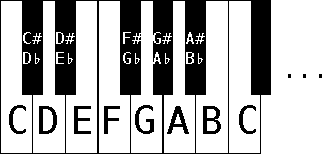
\includegraphics[width=0.6\linewidth]{Figures/piano-keys.pdf}
    \caption{Illustration of an octave in the 12-note chromatic scale
        on a piano keyboard.}
    \label{fig:piano-keys}
\end{figure}

Since pitch classes represent equivalence class of frequencies spaced an
integral number of octaves apart, unambiguously specifying a pitch requires not
only a pitch class but also an octave. In scientific pitch notation, this is
accomplished by appending an octave number to a pitch class letter (see
\autoref{fig:pitch-class}). Together, a pitch class and octave number uniquely
specify the notation for a pitch. On sheet music, the pitch of a note is
indicated by its vertical position with respect to the \emph{stave} (the five
horizontal lines and four spaces).

\begin{figure}[htpb]
    \centering
    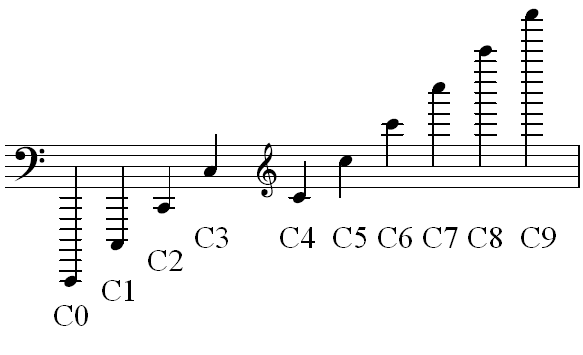
\includegraphics[width=0.6\linewidth]{Figures/Pitch_notation.png}
    \caption{Scientific pitch notation and sheet music notation of $C$ notes at
    ten different octaves.  \todo{Cite wiki scientific pitch notation}}
    \label{fig:pitch-class}
\end{figure}

Note that the discussion of pitch thus far has not made any direct connection
between pitch and frequency. Indeed, this lack of dependence on absolute
physical frequency highlights music's \emph{transposition invariance property}:
many semantically relevant features in music are present the relative relations
between pitches rather than absolute frequencies and hence remain invariant
when the entire piece of music is offset by a constant frequency. However, a
fixed reference frequency is oftentimes required for performance and
reproduction purposes. To convert from pitch notation to physical frequencies,
common modern practice is to tune $A4$ to 440 Hz (a practice known as A440).

In addition to pitch, a note also possesses a \emph{duration}. The duration of
a note indicates how long it is to be played and is measured in fractions of a
\emph{whole note} (American) or \emph{semibreve} (British). Perhaps the most
common duration is a \emph{quarter-note} (American) or \emph{crotchet}
(British). Other note durations are also possible and the most common along
with their notation in sheet music are enumerated in
\autoref{fig:note-durations}. The relationship between durations and
physical time intervals is given by the \emph{tempo}, which is usually
denoted near the start of the piece in beats per minute.

\begin{figure}[htpb]
    \centering
    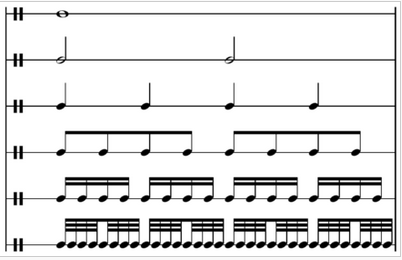
\includegraphics[width=0.6\linewidth]{Figures/note-durations.png}
    \caption{Comparison of various note durations. \todo{Cite wiki Whole note}}
    \label{fig:note-durations}
\end{figure}

Our work focuses in particular on \emph{tonal music}, a genre of music
characterized by the prevalence of one pitch class (the \emph{tonic}) around
which the melody and harmony are built.

A basic concept within tonal music is the \emph{scale}, which defines a subset
of pitch classes that are ``in key'' with respect to the tonic. Two fundamental
scales are the major (with step pattern
whole-whole-half-whole-whole-whole-half) and minor scales
(whole-half-whole-whole-half-whole-whole). The choice of tonic and scale is
collectively referred to as the \emph{key}. Many musical phenomena such as
stability, mood, expectation, and resolution can be attributed to choice of key
and \emph{modulations} (i.e. changes in key during the middle of a piece of
music).

\section{Neural sequence probability modeling}

Our work in later sections make heavy use of neural networks. In this section,
we briefly review the relevant concepts and set up notation.

\subsection{Neurons: the basic computation unit}

Neurons are the basic abstraction which are combined together to form
neural networks. A \emph{neuron} is a parametric model of a function $f : \RR^D \to
\RR$ from its $D$-dimensional input $\x$ to its output $y$. Our neurons will be
defined as
\begin{equation}
    f(\x) \coloneqq \sigma( \langle \vec{w}, \x \rangle)
\end{equation}
which can be viewed as an inner product with \emph{weights} $\vec{w}$ to
produce an \emph{activation} $z \coloneqq \langle \vec{w}, \x \rangle
\in \RR$ which is then squashed to a bounded domain by a non-linear
\textbf{activation function} $\sigma : \RR \to [L, U]$. This is visually
depicted in \autoref{fig:nn-single}, which also makes apparent the
interpretation of weight $w_i$ as the sensitivity of the output $y$ to the
input $x_i$.

\begin{figure}[htpb]
    \centering
    \input{Figures/nn-single.pdf_tex}
    \caption{A single neuron first computes an activation $z$ and then passes it through
    an activation function $\sigma(\cdot)$}
    \label{fig:nn-single}
\end{figure}

\subsection{Feedforward neural networks}

Multiple neurons may share inputs and have their outputs concatenated together
to form a \emph{layer} modelling a multivariate functions $f :
\RR^{D_\text{in}} \to \RR^{D_\text{out}}$. Multiple layers can then
be composed together to form a \emph{feedforwd neural network}.

\begin{figure}[htpb]
    \centering
    \input{Figures/nn-ffw.pdf_tex}
    \caption{Graph depiction of a feedforward neural network with $2$ hidden layers}
    \label{fig:nn-ffw}
\end{figure}

Although a single hidden layer is theoretically sufficient for a universal
function approximator\cite{Cybenko1993}, the number of hidden units to
guarantee reported theoretical bounds are usually unfeasibly large. Instead,
recent work in \emph{deep learning} has shown that deep models which contain
many hidden layers can achieve strong performance across a variety of
tasks\cite{Bengio2011}.

The improved modeling capacity gained by composing multiple layers is due to
the composition of multiple non-linear activation functions.
In fact, it is easy to show that removing activation functions would make
a deep network equivalent to a single matrix transform: let $\W_{l,l+1}$
denote the weights between layers $l$ and $l+1$. The original neural network
computes the function
\begin{equation}
    \sigma\left(
        \W_{L,L-1} \sigma \left(
            \W_{L-1,L-2}\cdots \sigma \left(
                \W_{2,1} \x
            \right) \cdots
        \right)
    \right)
\end{equation}
After removing the activation functions $\sigma$, we are left with
\begin{equation}
    \W_{L,L-1} \W_{L-1,L-2}\cdots \W_{2,1} \x
    = \x
    = \tilde{\W} \x
\end{equation}
where $\tilde{\W} = \left(\prod_{i=1}^{L-1} \W_{i,i+1} \right)$
is a matrix transform computing the same function as the neural network with
activation functions removed.

\subsection{Recurrent neural networks}

While feedforward neural networks provide a flexible model for approximating
arbitrary functions, they require a fixed-dimension input $\x$ and hence
cannot be directly applied to sequential data $\x = (x_t)_{t=1}^T$ where $T$ may
vary.

\todo{Introduce $\theta$ for parameters}

A naive method for extending feedforward networks would be to independently
apply a feedforward network to compute $y_t = f(x_t; \theta)$ at each timestep
$1 \leq t \leq T$. However, this approach is only correct when each output $y_t$
only depends on the input at the current time $x_t$. This assumption
is false in many scenarios: the current musical note depends on the sequence of
notes leading up to it.

This shortcoming motivates \emph{recurrent neural networks} (RNNs), which
generalize feedforward networks by introducing time-delayed recurrent
connections between hidden layers (Elman networks \cite{elman1990finding}) or
from the output layers to the hidden layers (Jordan networks
\cite{jordan1997serial}). \autoref{fig:nn-rnn} illustrates an Elman-type network:
note that apart from the edges between hidden nodes, the network is identical to
a standard network (\autoref{fig:nn-ffw}).

\todo{Why do we use Elman}

\begin{figure}[htpb]
    \centering
    \input{Figures/nn-rnn.pdf_tex}
    \caption{Graph depiction of an Elman-type RNN. Note the recurrent connections
    within the hidden layer.}
    \label{fig:nn-rnn}
\end{figure}

\autoref{fig:rnn-elman} reinterprets the recurrent hidden layer connections in
\autoref{fig:nn-rnn} as inputs whose values are taken from the previous hidden
state making the time-delay explicit. Additionally, \autoref{fig:rnn-elman}
introduces the notion of \emph{memory cells}, which abstract the internals
of RNNs into a computational unit which for each timestep $t$:
\begin{itemize}
    \item Takes as inputs
        \begin{itemize}
            \item The current element in the input sequence $\x_t$
            \item The previous hidden state $\h_{t-1}$
        \end{itemize}
    \item Produces the outputs
        \begin{itemize}
            \item The updated hidden state $\h_t = f_h (\x_t, \h_{t-1})$
            \item The outputs $\y_t = f_y (\h_t)$.
        \end{itemize}
\end{itemize}

\begin{figure}[htpb]
    \centering
    \input{Figures/nn-rnn-elman.pdf_tex}
    \caption{Equivalent formulation of an Elman-type RNN treating the time-delayed hidden state
    as additional inputs to a feedforward network}
    \label{fig:rnn-elman}
\end{figure}

The memory cell abstraction is convenient because it enables discussion of RNN
architecture without settling on a particular memory cell implementation. In
particular, it enables us to \emph{unroll the RNN} by removing the time-delayed
recurrent cycle and replicating the memory cell over multiple timesteps as seen
in \autoref{fig:rnn-single-unrolled}. This gives rise to a finite directed
acyclic graph where nodes represent pieces of data and edges $s \to t$ indicate
that $t$ is a function of $s$.

It is interesting to note the similarity between unrolled RNN and feedforward
networks: both are acyclic and the semantic meaning of the nodes and edges are
identical. In fact, one can view an unrolled RNN as a feedforward network with
as many layers as the elements in the input sequence $(\x_t)_t$ and
parameters tied across all layers. This similarity has inspired fruitful
cross-polination in both fields: methods for training feedforward networks have
been adapted to RNNs and methods for learning long timespan dependencies in
RNNs have been used to train even deeper neural networks. \todo{Foreshadow, or
use as a transition}. \todo{Depth in time makes training difficult, similar to
    DNNs. LSTM inspires highway networks for DNNs DNNs and grid-LSTMs for deep
LSTMs}

\begin{figure}[htpb]
    \centering
    \input{Figures/rnn-single-unrolled.pdf_tex}
    \caption{Signal flow diagram representation of a single-layer RNN and its corresponding
    expansion into a computation graph}
    \label{fig:rnn-single-unrolled}
\end{figure}

\autoref{fig:rnn-single-unrolled} makes it obvious how the hidden state is
carried along throughout the sequence of computations, giving rise to a useful
alternative interpretation of the hidden state as a temporal memory mechanism.
Under this interpretation, we can view the hidden state update $\h_t = f_h
(\x_t, \h_{t-1})$ as \emph{writing} information extracted from the
current inputs $\x_t$ to the memory $\h_{t-1}$. Similarly, producing
the outputs $\y_t = f_y (\h_t)$ can be seen as \emph{reading}
information from the hidden state.

\todo{Compare to N-grams; show how it's like an infinite context. One
    interpretation is to view the hidden state $\h_t$ as an
    infinite-length prior context window, summarizing all of the prior inputs
    into into a compact fixed-size vector.}

Since the RNN outputs $\y$ also form a sequence with the same length as
the inputs $\x$, they can be used as inputs into another RNN. This
stacking of multiple memory cells is similar to the layering seen in deep
neural networks, giving rise to the term \emph{deep neural sequence models}
\todo{Cite?}. This is illustrated in \autoref{fig:rnn-multi-unrolled}.

\begin{figure}[htpb]
    \centering
    \input{Figures/rnn-multi-unrolled.pdf_tex}
    \caption{Unrolled computation graph for a 2-layer RNN}
    \label{fig:rnn-multi-unrolled}
\end{figure}

The greater modeling capabilities of multilayer RNNs can be attributed to two
primary factors: composition of multiple non-linearities and an increase in the
number of paths through which information can flow. The former is analogous to
the feedforward case: stacking memory cells increases the number of
non-linearities in the composite cell just like stacking multiple layers in
feedforward networks. To understand the latter point, notice that in
\autoref{fig:rnn-single-unrolled} there is only a single path from
$\x_{t-1}$ to $\y_{t}$ hence the conditional independence
$\y_{t} \independent \x_{t-1} | \h^{(1)}_t$ is satisfied.
However, in \autoref{fig:rnn-multi-unrolled} there are multiple paths from
$\x_{t-1}$ to $\y_{t}$ (e.g. passing through either
$\h^{(2)}_{t-1} \to \h^{(2)}_t$ or $\h^{(1)}_{t-1} \to
\h^{(1)}_t$) through which information may flow. Additionaly, the
hidden state transitions occur on two seperate memory cells so parameters
need not be tied and the stacked RNN can learn different time dynamics
at each depth.

\subsection{Training RNNs and backpropogation through time}

Mathematically, we may define a RNN as a discrete time dynamical system:
One standard parameterization is
\begin{eqnarray}
    \h_t &=& \W_{xh} \sigma_{xh} \left( \x_t \right) + \W_{hh} \sigma_{hh} \left( \h_{t-1} \right) \\
    \y_t &=& \W_{hy} \sigma_{hy} \left( \h_t \right) \\
\end{eqnarray}
where $\sigma_{\cdot}(\cdot)$ are activation functions acting element-wise
and the parameters $\theta = \{ \W_{xh}, \W_{hh}, \W_{hy}\}$
are learned from data to minimize a cost $\mathcal{E} = \sum_{1 \leq t \leq T}
\mathcal{E}_t(\x_t)$ measuring the performance of the network on some task.

One approach for computing the necessary gradients is \emph{backpropogation through
time} (BPTT)\cite{At}, an adaptation of the backpropogation algorithm \todo{cite}
to the unrolled RNN computation graph. Letting $\theta$ denote the model parameters,
we can apply the chain rule to the unrolled RNN's computation graph
in \autoref{fig:rnn-bptt} to obtain
\begin{eqnarray}
    \frac{\pd \mathcal{E}}{\pd \theta} &=& \sum_{1 \leq t \leq T} \frac{\pd \mathcal{E}_t}{\pd \theta} \\
    \frac{\pd \mathcal{E}_t}{\pd \theta} &=& \sum_{1 \leq k \leq t} \left(
        \frac{\pd \mathcal{E}_t}{\pd \y_t}
        \frac{\pd \y_t}{\pd \h_t}
        \frac{\pd \h_t}{\pd \h_k}
        \frac{\pd \h_k}{\pd \theta}
    \right) \label{eq:error-t}\\
    \frac{\pd \h_t}{\pd \h_k} &=&
    \prod_{t \geq i > k} \frac{\pd \h_i}{\pd \h_{i-1}}
    = \prod_{t \geq i > k} \W_{hh}^\tp \diag \left( \sigma_{hh}'( \h_{i-1} ) \right)
    \label{eq:error-transfer}
\end{eqnarray}

\begin{figure}[htpb]
    \centering
    \input{Figures/rnn-bptt.pdf_tex}
    \caption{The gradients passed along network edges during BPTT.}
    \label{fig:rnn-bptt}
\end{figure}

\autoref{eq:error-t} expresses how the error $\mathcal{E}_t$ at time $t$ is a sum
of \emph{temporal contributions} $
\frac{\pd \mathcal{E}_t}{\pd \y_t}
\frac{\pd \y_t}{\pd \h_t}
\frac{\pd \h_t}{\pd \h_k}
\frac{\pd \h_k}{\pd \theta}$
measuring how $\theta$'s impact on $\h_k$ affects the cost at some future
time $t > k$. The factors in \autoref{eq:error-transfer} measures the affect
of the hidden state $\h_k$ on some future state $\h_t$ where $t > k$
and can be interpreted as transferring the error ``in time'' from step $t$ back
to step $k$ \cite{Pascanu2012}.

\subsubsection{Vanishing/exploding gradients}

Unfortunately, the formulation of RNNs as presented in \todo{reference section}
suffers from two well known problems: the \emph{vanishing gradient} and
\emph{exploding gradient}\cite{Bengio1994}. Broadly speaking,
these problems are both related to the product in \autoref{eq:error-transfer}
exponentially growing or shrinking for long timespans (i.e. $t \gg k$).

Following Pascanu \textit{et al.} \cite{Pascanu2012}, let $\| \cdot \|$ be any
submultiplicative matrix norm (e.g. Frobenius, spectral, nuclear, Shatten
$p$-norms). Without loss of generality, we will use the \emph{operator norm}
defined as
\begin{equation}
    \| A \| = \sup_{x \in \RR^n; x \neq 0} \frac{|A x|}{|x|}
\end{equation}
where $|\cdot|$ is the standard Euclidian norm.

From submultiplicativity, we have that for any $k$
\begin{equation}
    \left\| \frac{\pd \h_k}{\pd \h_{k-1}} \right\|
    \leq \| \W_{hh}^\tp \| \| \diag\left( \sigma_{hh}'(\h_{k-1}) \right) \|
    \leq \gamma_{\W} \gamma_\sigma
\end{equation}
where we have defined $\gamma_{\W} = \| \W_{hh}^\tp \|$ and
\begin{align}
    \gamma_\sigma
    &\coloneqq \sup_{h \in \RR^n} \| \diag \left( \sigma_{hh}'(\h) \right) \|  &\\
    &= \sup_{h \in \RR^n} \max_i \sigma_{hh}'(\h)_i &\mbox{Operator norm of diag} \\
    &= \sup_{x \in \RR} \sigma_{hh}'(x) &\mbox{$\sigma_{hh}$ acts elementwise}
\end{align}

Substituting back into \autoref{eq:error-transfer}, we find that
\begin{equation}
    \left\| \frac{\pd \h_t}{\pd \h_k} \right\|
    = \left\| \prod_{t \geq i > k} \frac{\pd \h_i}{\pd \h_{i-1}} \right\|
    \leq  \prod_{t \geq i > k} \left\| \frac{\pd \h_i}{\pd \h_{i-1}} \right\|
    \leq (\gamma_{\W} \gamma_\sigma)^{t-k}
\end{equation}

Hence, we see that a sufficient condition for vanishing gradients is
for $\gamma_{\W} \gamma_\sigma < 1$, in which case $\left\| \frac{\pd \h_t}{\pd \h_k} \right\| \to 0$
exponentially for long timespans $t \gg k$. $\qed$

For common activation functions, $\gamma_\sigma$ is bounded and reasonably
small (e.g. $\gamma_\sigma = 1$ for $\sigma_{hh} = \tanh$, $\gamma_\sigma =
0.25$ for $\sigma_{hh} = \sigmoid$). This enables us to write the sufficient
condition for vanishing gradients as
\begin{equation}
    \gamma_{\W} = \| \W_{hh}^\tp \| \leq \frac{1}{\gamma_\sigma}
    \label{eq:vanishing-gradients-suff}
\end{equation}
The converse of the proof implies that $\| \W_{hh}^\tp \| \geq
\frac{1}{\gamma_\sigma}$ are necessary conditions for $\gamma_{\W}
\gamma_\sigma > 1$ and exploding gradients to occur.

\subsection{Long short term memory}

As \autoref{eq:vanishing-gradients-suff} provide sufficient conditions for
vanishing gradients, any model which we may hope to successfuly learn long range
dependencies must have $\gamma_{\W} \gamma_\sigma \geq 1$.

The \emph{long short term memory} (LSTM) model was proposed by Hochreiter and
Schmidhuber \cite{hochreiter1997long} as a method for dealing with
the vanishing gradient problem. It does so by enforcing \emph{constant error flow}
on \autoref{eq:error-transfer}, that is
\begin{equation}
    \W_{hh}^\tp \sigma_{hh}' (\h_{t}) = \matr{I}
\end{equation}
where $\matr{I}$ is the identity matrix.

Integrating the above differential equation yields $\W_{hh} \sigma_{hh}(\h_{t}) = \h_{t}$.
Since this should hold for any hidden state $\h_{t}$, this means that:
\begin{enumerate}
    \item $\W_{hh}$ must be full rank
    \item $\sigma_{hh}$ must be linear
    \item $\W_{hh} \circ \sigma_{hh} = \matr{I}$
\end{enumerate}
In LSTMs, this is ensured by setting $\sigma_{hh} = \W_{hh} = \matr{I}$, effectively removing
time dynamics from the hidden state. In the literature, this is referred to as
the \emph{constant error carousel} (CEC).

In addition to the CEC \todo{which is also seen in xyz}, LSTMs possess three sets of gates controlling
access to the CEC:
\begin{itemize}
    \item \textbf{Input gate}: scales input $x_t$ elementwise by $i_t \in [0,1]$, affects how $h_t$ is written to
    \item \textbf{Output gate}: scales output $y_t$ elementwise by $o_t \in [0,1]$, affects how $h_t$ is read from
    \item \textbf{Forget gate}: scales previous cell value $h_{t-1}$ by $f_t \in [0,1]$, acts as a reset mechanism
\end{itemize}
\todo{Discuss how the three gates are used}

\autoref{fig:lstm-cell} depicts a single LSTM cell. Notice that it adheres

\begin{figure}[htpb]
    \centering
    \input{Figures/lstm-unit-2.pdf_tex}
    \caption{Schematic for a single LSTM cell.}
    \label{fig:lstm-cell}
\end{figure}

\begin{eqnarray}
    \i_t &=& \sigmoid(\W_{xi} \x_t + \W_{yi} \y_{t-1} + \b_i) \\
    \o_t &=& \sigmoid(\W_{xo} \x_t + \W_{yo} \y_{t-1} + \b_o) \\
    \f_t &=& \sigmoid(\W_{xf} \x_t + \W_{yf} \y_{t-1} + \b_f) \\
    \h_t &=& \f_t \odot \h_{t-1} + \i_t \odot \tanh(\W_{xh}\x_t + y_{t-1} \W_{yh} + \b_h) \label{eq:lstm-dynamics} \\
    \y_t &=& \o_t \odot \tanh(\h_t)
\end{eqnarray}
where $\odot$ denotes elementwise multiplication of vectors.

Note that \autoref{eq:lstm-dynamics} has $\phi$ set to the identity function
hence $\gamma_\phi = 1$. This removal of the non-linearity in the hidden state
recursion is known as the \textbf{constant error carousel} \todo{cite}, which
allows the network to propogate errors without modification by $\varphi'(h_k)$.

The addition of the gates enables the model to learn when to read/write from
memory and when to reset, enabling longer-range dependencies to be learned when
an input is written to memory (i.e. $i_t$ high) and protected for a long
duration (i.e. $f_t \approx 1$ and $i_t \approx 0$).

Some authors define LSTMs such that $h_t$ is not used to compute gate activations,
referring to the case where $h_t$ is connected as ``peephole connections.'' In our
work, we use ``LSTM'' to refer to LSTMs with peephole connections.

LSTMs protect from vanishing gradient, but not exploding gradient. Research has shown
that gradient clipping is essential to permit successful applications \cite{Pascanu2012}.
\begin{enumerate}
    \item 
\end{enumerate}

\todo{Truncated BPTT}
\todo{Gradient clipping for avoiding exploding gradient}

\subsubsection{Sequential processing and sampling}

We will train our RNNs to predict a distribution for the next character
$\x_{t+1}$ after the RNN has processed the sequence $\x_{1:t}$,
yielding a model which factorizes the sequence probability
\begin{equation}
    P(\x_{1:T}) = \prod_{t=1}^T P(\x_t | \x_{1:t-1} )
\end{equation}
Modeling this probability distribution over sequences is analogous to the
\textbf{language modeling} from speech recognition.

Note that the factorization of conditional distributions \emph{assumes a
sequential ordering in $t$}. This property is desirable as it enables sampling
from the model to generate new transcriptions by sampling from $P(\x_t |
\x_{1:t-1})$ at each timestep $t$ and using the sampled value as the next
input.

\todo{compare to bidirectional}.

\todo{for more details, see XYZ}.

\subsection{Parameter estimation of recursive neural networks}

\subsubsection{Modeling probabilities using the Boltzmann distribution and cross-entropy error criterion}

The parameters to the model are estimated in order to minimize the error
between the network outputs and provided labels. For language modeling, the
outputs $\y_t$ should parameterize a distribution for the next character
$P(\x_{t+1} | \x_{1:t})$. Suppose each input has finite support (i.e.
$\x_t \in [1,2,\cdots,K]$). If we choose the outputs to be $K$ dimensional
(i.e. $\y_t \in \RR^K$) then the \textbf{Boltzmann distribution}
(\autoref{eq:boltzmann-dist}) can be used:

\begin{equation}
    \label{eq:boltzmann-dist}
    P(\x_{t+1} = s | \x_{1:t})
    = \frac{\exp \left(-\y_{t,s}/T\right) }{ \sum_{k=1}^{K} \left(\exp -\y_{t,k}/T\right)}
\end{equation}

$T \in \RR^+$ is a \textbf{temperature} parameter \todo{relate to sampling}.

The labels provided are the actual next characters $\x_{t+1}$. Viewing
such labels as discrete probability distributions will all mass on a single atom,
one measure of difference between predictions and \todo{justify cross-entropy}

\documentclass[dissertation.tex]{subfiles}
\begin{document}

\chapter{Related Work}
% This chapter covers relevant (and typically, recent) research
% which you build upon (or improve upon). There are two complementary
% goals for this chapter:
% \begin{enumerate}
%   \item to show that you know and understand the state of the art; and
%   \item to put your work in context
% \end{enumerate}

% Ideally you can tackle both together by providing a critique of
% related work, and describing what is insufficient (and how you do
% better!)

% The related work chapter should usually come either near the front or
% near the back of the dissertation. The advantage of the former is that
% you get to build the argument for why your work is important before
% presenting your solution(s) in later chapters; the advantage of the
% latter is that don't have to forward reference to your solution too
% much. The correct choice will depend on what you're writing up, and
% your own personal preference.

% Some common themes
% \begin{enumerate}
%   \item Use of domain-specific representations for musical data
%   \item Modeling at multiple resolutions / timescales (i.e. chords vs notes)
% \end{enumerate}
% In contrast, we avoid imposing prior knowledge in order to avoid any biases
% and hope that the model will learn the features relevant for good performance.

\section{Machine learning on musical data}

Computational methods applied to large corpuses of music was first described in
\cite{coutinho2005computational}, which termed the phrase ``computational
musicology.'' Since then, development modern tools have greatly aided research
efforts. \texttt{music21} \cite{Scott2015} is a Python programming environment
for performing computations over musical composition data which has been
utilized for a variety of computational musicology tasks ranging from
heirarchical modeling of metrical structure \cite{ariza2010modeling}, feature
generation for downstream machine learning\cite{Cuthbert2011}, and style
classification \cite{Herlands2014}.

Focusing on machine learning applications, most research can be
classified under one or more of the following tasks:
\begin{enumerate}
  \item Classification: the style, composer, or other musical attribute is to be classified
  \item Harmonization: a melody is given and the remaining parts are to be generated
  \item Completion: given the beginning of a score, the remainder is to be generated
  \item Automatic Composition: a complete unconstrained score is to be generated
\end{enumerate}

There is a vast body of research dealing with music classification tasks,
including: style classification \cite{Herlands2014}
\cite{dannenberg1997machine}, automated harmonic analysis \cite{ni2012end},
information retrieval \cite{mandel2006support}, and performer identification
\cite{stamatatos2005automatic}. However, it is not straightforward to utilize
work in this area to solve our research goals of music synthesis\todo{of what?}.

\section{Models for music synthesis}

Unlike classification, the other tasks (harmonization, completion, automatic
composition) require synthesis of novel music. One broad classification of
music synthesis methods \cite{toiviainen2000symbolic} distinguishes between
symbolic (i.e. rule based) versus connectionist (i.e. neural networks).

\subsection{Symbolic rule-based methods}

CHORAL \cite{ebciouglu1988expert} is one of the first rule based expert system
for harmonizing Bach chorales. It uses 350 manually defined rules as well as
hand-tuned search heuristics. A later system called \emph{Experiments in Music
Intelligence} (EMI) \cite{cope1992computer} automatically extracted rules to
build an augmented transition network\cite{wanner1980atn}. In
\cite{cruz1998learning}, grammatical inference is used to learn regular
grammars over chord progressions for modeling musical style.
\cite{tsang1991harmonizing} applies constraint logic programming for generating
harmonizations which satisfy certain harmonic constraints.

While symbolic methods can easily incorporate domain-specific knowledge and are
more interpretable than connectionist models, they are also inherently biased
by their creators' subjective theories on harmony and music cognition.
Furthermore, specification of hand-crafted rules is a laborious process which
requires significant music experience and does not improve when given larger
amounts of data. Additionally, rule-based methods are brittle to distortion and
noise and limit creativity by disallowing deviation from the defined rules.

\subsection{Connectionist methods}

Neural networks have been previously applied to music with varying degrees of
success\cite{griffith1999musical}. The earliest connectionist music models
utilized note-level Jordan RNNs on melody generation and harmonization tasks
\cite{todd1988sequential} \cite{todd1989connectionist}
\cite{bharucha1989modeling}. \todo{say more}

A landmark connectionist system is Mozer's CONCERT \cite{mozer1994neural}, a
BPTT RNN for note-by-note composition. CONCERT models music at two
levels of resolution: notes and chords. Notes utilize a psychologically-based
representation \cite{shepard1982geometrical} and chords use a distributed
embedding originally trained for style classification
\cite{laden1989representation}. The model passes objective evaluations by
faithfully reproducing scales but ``while the local contours made sense, the
pieces were not musically coherent, lacking thematic structure and having
minimal phrase structure and rhythmic organization`` \cite{mozer1994neural}.

\cite{Boulanger-Lewandowski2012} proposed the RNN-RBM. a time-varying RBM with
hidden units evolving over time according to a RNN, to model polyphonic music
on a piano roll representation. However, training the RNN-RBM requires an
expensive contrastive divergence sampling step at each timeframe and a
nontrivial Hessian-free optimization routine. Furthermore, the authors
quantized music to eigth-notes. In contrast, our work uses the well-understood
truncated BPTT algorithm for training and quantizes to sixteenth-notes to achieve
two-times higher time resolution.

\cite{Lyu2015} extended the RNN-RBM\cite{Boulanger-Lewandowski2012} to use a
LSTM instead of a RNN for modeling hidden unit time dynamics. Unfortunately,
the authors do not evaluate their model beyond stating ``LSTM-RTRBM could learn
melody lines\ldots while RTRBM generates incosistent and unpleasant sample
sequences.''

\subsection{Hybrid methods}

Hybrid approaches which combine both rule-based and connectionist methods have
also been investigated. One of the first hybrid systems for music synthesis is
HARMONET \cite{hild1991harmonet}, which combines connectionist neural networks
with formal rules to specifically harmonize Bach chorales. It implements a
domain-specific processing pipeline consisting of:
\begin{enumerate}
  \item Harmonic modelling: Predict harmonic skeleton (i.e. Roman numerals
  quantized to quarter-notes) using a neural network
  \item Expand each Roman numeral to chords using formal rules
  \item Ornamentation: add eigth-notes using formal rules
\end{enumerate}
The specialized architecture of HARMONET makes it unable to generalize
to other tasks such as automatic composition or composition scoring\todo{Define this task}.
Additionally, the use of formal rules makes the system suffer from the same
problems that rule-based systems suffer from.

MELONET \cite{feulner1994melonet} builds on top of HARMONET's harmonic
modelling to construct chorale partitas (i.e. variations where one of the
parts is varied in a harmonically believable way). It first introduced multiple
ideas which have been rediscovered in recent years, including:
\begin{enumerate}
  \item Delayed update units to model multiple timescales (described again in Clockwork
  RNNs \cite{Koutnik2014})
  \item Use of Resilient Propogation (RProp) \cite{riedmiller1993direct} for training (
  described again in \cite{Liu2014})
\end{enumerate}
Additionally, MELONET utilizes a motif classification neural network to
explicitly force motifs to appear multiple times within a partita.
Follow up work \cite{hornel1996learning} extends MELONET to use a distributed
representation for motifs and a genetic algorithm for training.
While MELONET introduces many novel ideas, its limited training set size
(16 Pachelbel chorales \cite{hornel1997melonet}) and domain-specific
architecture limit the generalizability of results. \todo{Better analyze this}

CHIME \cite{franklin2001learning} adopted the Jordan RNN from
\cite{todd1989connectionist} to add a second training phase using actor-critic
reinforcement learning \cite{sutton1998reinforcement}. The critic is
constructed using a collection of ``music rules,'' enabling incorporation of
prior knowledge.

\subsection{LSTM music synthesis models}

Prior work has demonstrated LSTM possesses many properties desirable for music
applications. Their superiority over traditional RNNs has been well
documented\cite{gers2001lstm}. They can learn to count and measure time
intervals between events spaced arbitrarily far apart in time
\cite{gers2000recurrent}, a property $N$-gram language models do not possess.
\cite{gers2002learning} demonstrated LSTM learning to produce self-sustaining
oscillations at a regular frequency, suggesting that they are capable of
discovering periodic structure. \cite{franklin2006recurrent} evaluates various
RNN architectures on variety of music tasks and concludes: ``while we have
found a task that challenges a single LSTM network, we do not believe that any
other recurrent networks we have used would be able to learn these songs.'''

One of the first applications of LSTMs to music was to improvize blues melody
lines \cite{Eck2002}\cite{Eck2002-blues}. Using a LSTM to model blues chord
progressions and another to model melody lines given chords, the authors
reported that LSTM can learn long term music structure such as repeated motifs
can be learned without explicit modeling (e.g. MELONET). However, the music
representation quantized to 8th notes, used considered pitch classes without
accounting for octaves, and limited the model to $12$ possible chords.
Additionally, there was ``no explicit way to determine when a note ends,''
prohibiting discrimination between four consecutive articulations of a note at
the same pitch from a single note held for four timesteps. In contrast, our
model accounts for the octaves in addition to pitch class, does not restrict
the possible chords, operates at twice the time resolution, and also
models when a note ends.

More recently, \cite{sturm2015folk} \cite{sturm2016music} trained
character-level LSTMs on 23,000 folk music scores represented in ABC
notation\cite{abcstandard}, a high-level text format for music. ABC format is
unsatisfactory for our use case because polyphonic scores are encoded one part
at a time so notes sounding close together in time may appear very far apart in
the sequence. As a result, it is unsurprising that the authors do not
explicitly address polyphony and present exclusively monophonic results.

Many variants of the LSTM architecture have been proposed. Perhaps the most
well known is the gated recurrent unit (GRU)\cite{cho2014learning}, which
constrains the input and forget gates to sum to $1$. \cite{Mikolov2015}
proposed the structurally cosntrained RNN (SCRN), a simple architecture
achieving comparable performance to LSTMs. Of most relevance to music,
\cite{Koutnik2014} proposed the clockwork RNN for explicitly modeling phenomena
occuring at multiple timescales by updating different blocks of the hidden
state at different periods. Whether these differences matter is not definitive:
\cite{greff2015lstm} performed 5400 experiments on eight different
architectures and found no significant difference in performance compared to
the original LSTM architecture. \cite{Nayebi2015} reports LSTMs significantly
outperform GRUs in music applications.

\section{Generative modeling of Bach Chorales}

One of the first generative models for harmonizing Bach chorales is Bellgard
and Tsaing's effective Boltzmann machine model \cite{bellgard1994harmonizing}. Their model
uses Boltzmann machines to enforce consistency within local contexts. As a result,
their model is unable to capture long-range dependencies. Furthermore, they quantize
to half-notes and only achieve $1/8$ the time resolution of our model.

\cite{Allan2005} used HMMs to harmonize Bach chorales. Their model consists of
two separate HMM models: one for generating harmonizations and another for
ornamentation. Their model uses a discrete harmonic encoding of chords for
hidden states. In contrast, our model uses an unconstrained continuous hidden
state and requires no separate ornamentation step.

\cite{Liu2014} applied LSTMs to Bach chorales and reports significant gains
using RProp instead of BPTT, a technique previously utilized by
MELONET\cite{feulner1994melonet}. However, they erroneously use a mean squared
error training criterion for a classification task, casting doubts on the
validity of their experiments.

\cite{Brien2016} compared RNN models for Bach chorales and found clockwork RNNs to
yield the lowest validation loss. However, their data format does not permit
independent articulation of parts. More importantly, the performance margin between
clockwork RNNs and LSTMs was very small ($6.5$ vs $6.75$ cross-entropy loss) and their
implementation resets the LSTM state when truncating gradients during BPTT, limiting the
time-range of learned dynamics to be at most the sequence length.


\printbibliography

\end{document}

\chapter{Data}

We use a corpus of Bach chorales provided by \texttt{music21}. The chorales are
arranged by the Bach-Werke-Verzeichnis (BWV) numbering system, which is one of
the best known and widely used catalogues of Bach's compositions.

Each chorale has four parts and are structured such that the melody is in
the Soprano part and the remaining parts harmonize the melody.

\section{Preprocessing}

We transpose all scores with major key signatures to C major and minor key
signatures to A minor. Due to transposition invariance of 12-TET, this does
not alter the tonal properties of the music.

We represent musical scores using a piano roll representation. Firstly, time is
discretized into constant timestep frames. For each frame, a set of (note, tie)
pairs representing which a note's pitch and whether it is tied
(continuing a note from the previous frame) or newly played notes.

\begin{enumerate}
    \item Transpose to Cmaj/Amin
    \item Strip all dynamics info
    \item Restrict to 4/4
\end{enumerate}

Both frame-based processing and quantization to eighth notes justified by Eck
and Smidhuber LSTM Blues \todo{cite}. Eight network time steps are required to
process a whole note. This is preferrable for the LSTM because it forces the network to learn
relative duration of notes, making it easier for counting and timing mechanisms
to be encoded by the LSTM dynamics \todo{Cite Gers and Schmidhuber, 2000}.

\textbf{Contribution}: solved problem of determining when notes end (\todo{cite
Eck Schmidhuber LSTM blues}) in input data format by using the ties.



\chapter{Sequence probability modelling}

Generating a "Bach-like" piece of music can be understood as drawing a random
sample from a distribution over musical scores which is statistically similar
to Bach's own compositions. Thus, we interpret the problem as one of
\emph{categorical sequence modeling}.

This type of problem has been well studied. In speech recognition, language
models parameterizing distributions over sentences are used as priors to refine
transcriptions.

However, since our model has to be able to generate Bach, we must be able to
sample from it. This rules out a broad class of sequence models, including
back-off N-grams and other interpolated language models.

Fortunately, low order N-grams and standard HMM-based models are sampleable and
thus can be used as baselines.

\section{Feedforward neural networks}

Increasing context window size is not always a good solution:
\begin{itemize}
    \item Too small $\implies$ no long-term dependencies captured
    \item Not all $N$-grams observed $\implies$ need back-off and discounting
\end{itemize}

How do we handle variable length inputs?

\section{Recursive neural networks}

Carry memory $s_t$ through time $t$, ``summary of infinite context duration
i.e.\ all previously processed data''

Share weights $\matr{U}, \matr{V}, \matr{W}$ over $t$ since performing same
task at each time i.e.\ modeling $P(o_t | s_t, x_t) = \softmax(V s_t)$.

\begin{figure}[htpb]
    \centering
    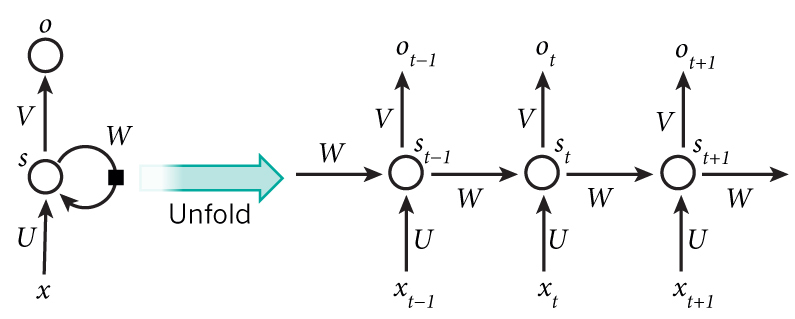
\includegraphics[width=0.8\linewidth]{Figures/rnn.jpg}
    \caption{\todo{Redraw in xy}}
\end{figure}

\begin{align}
    \s_t &= f(\U \x_t + \W \s_{t-1}) \\
    \o_t &= \softmax( \V \s_t)
\end{align}

$f$ is usually $\tanh$ or ReLU.

\begin{enumerate}
    \item Memory/state $\s_t$ summarizes ALL previous information
    \item $\U, \V, \W$ parameters are shared across all $t$. Reflects
        that the same task is being performed at each input i.e.\
        invariance over time. Reduces number of parameters.
\end{enumerate}


RNNs are a sequence model similar to HMMs in that they model the conditional
distribution of next frames given the previous context. However, RNNs additionally
pass along "hidden state" which summarizes contextual information from a potentially
infinite context window.

In practice, it is observed that the hidden state does not capture long range
dependencies well and tend to suffer from vanishing/exploding gradient during
training. LSTMs are an improved RNN architecture which solve both of these
problems by introducing gates on the inputs, hidden state, and outputs. GRUs are
a variation of LSTMs which ties the weights to the input and forget gates.

\begin{enumerate}
    \item Language modeling
        \begin{enumerate}
            \item Model $P(\m), \m \in V^T, T \in \NN$
            \item Train to predict the distribution of the next note in the
                melody i.e.\ $\o_t = P(\m_t | \m_{1:t-1})$
            \item $\m_{t-N:t-1}$ is given explicitly as input $\x_t$ and
                $\s_{t}$ captures information from before $t-N$
            \item See \cite{Martens2011}, \cite{Mikolov2011}, \cite{Mikolov2010}
        \end{enumerate}
    \item Machine translation
        \begin{enumerate}
            \item~\\
                \begin{figure}[htpb]
                    \centering
                    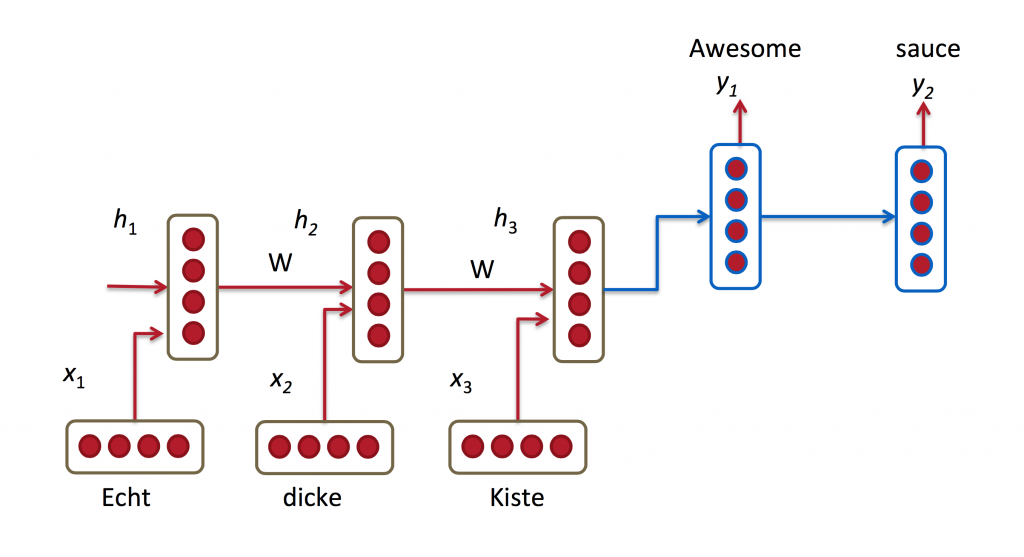
\includegraphics[width=0.8\linewidth]{Figures/rnn-mt.png}
                    \caption{\todo{Redraw in xy}}
                \end{figure}
            \item Input is a sequence of words in source language $\leftrightarrow$
                sequence of notes in $V$
            \item Output is four sequences of notes, one for each of the 4 chorale parts.
            \item Architecture difference: output only starts after input is completely
                consumed because first word of translated sentence may require information
                from complete sentence input
                \begin{enumerate}
                    \item This could be mitigated with bidirectional LSTMs \cite{Graves2005}
                    \item Could also try Neural MT \cite{Bahdanau2015}, whose attention
                        neural network could be used to extract insights about which parts
                        of the overall melody influences decision making within local regions
                        of music
                \end{enumerate}
            \item See \cite{Liu2014}, \cite{Auli2013}, \cite{Sutskever2014}.
        \end{enumerate}
\end{enumerate}


\documentclass[dissertation.tex]{subfiles}
\begin{document}

\chapter{Chorale harmonization}

\todo{Talk about how correct harmonization is equivalent to conditioning on
  future hidden state over all possible $\h$ trajectories passing through it.
  Intractable conditioning, so we approximate by neglecting to constrain (i.e.
  don't account for future at all) and instead do teacher forcing. Hope that
  teacher forcing induces the hidden state to go in a reasonable trajectory,
but results show otherwise}


Unlike automatic composition, in harmonization tasks we are given the entire sequence of notes
for one or more parts. As one of the parts is now fixed, the model is no longer able to freely
compose and harmonic deviations from the fixed parts will result in dissonances and conflicting
expectations. This lack of accountability for future expectations is one of the failure modes of our models.
One potential method for mitigating this is bidirectional LSTMs\cite{Graves2005}, which account
for both the future and prior contexts. However, a bidirectional LSTM cannot be sequentially
sampled to perform automatic composition.

\section{Background}

A chorale consists of four parts: soprano, alto, tenor, and bass. Chorale harmonization
involves producing the alto, tenor, and bass parts given a fixed soprany melody. As described
by Walter Piston \cite{piston1978harmony}:

\begin{quote}
  True harmonisation, then, means a consideration of the alternatives in available chords, the reasoned selection of one
  of these alternatives, and the tasteful arrangement of the texture of the added parts with due regard
  for consistency of style
\end{quote}

The Baroque style employed by Bach has specific guidelines
such as disallowing parallel fifths and parallel octaves as well as
considerations for voice leading \cite{piston1978harmony}.

For a music student studying chorale harmonization, a common pedagogical
exercise \cite{denny1960oxford}\cite{piston1978harmony} is a sequence of tasks increasing in difficulty:
\begin{enumerate}
  \item Providing either alto and tenor given fixed soprano and bass
  \item Providing both alto and tenor parts given fixed soprano and bass
  \item Providing all remaining parts given only the soprano line
\end{enumerate}

There are no definitive formalization of the harmonization process, making
evaluation difficult. Attenpts to formalize the process using Shenkerian
structural analysis \cite{oswald1973harmony} and symbolic methods such as
generative grammars \cite{lerdahl1983jackendoff}\cite{winograd1968linguistics}
exist, but involve human analytical process.

\section{Harmonizing}


For chorale harmonization, we are interested in predicting the notes for a part
given the other parts. Concretely, suppose we wish to predict a $L \in \NN$
length sequence $w_{1:L}$. Let $\alpha \subset [1,T]$ be a multi-index,
$\alpha^c \coloneqq [1,T] \setminus \alpha$, and $w_\alpha$ the tokens
corresponding to the given parts. We are interested in finding
\begin{equation}
  w_{1:L}^* = \argmax_{w_{1:L}} P(w_{1:L} | w_{\alpha})
\end{equation}


``Clamp'' the generative model and have it ``fill-in'' missing bits
\cite{hinton1986learning}. We can constrain the set of candidate sequences by
first noting any solution $\hat{w_{1:L}}$ must satisfy $\hat{w}_\alpha =
w_\alpha$. We can apply this constraint and greedily sample from our generative
model to approximately solve the problem:
\begin{equation}
  \hat{w_{t}} = \begin{cases}
    w_{\alpha_t} &\mbox{if}~t \in \alpha \\
    \argmax_{w_t} \hat{P}(w_t | \hat{w}_{1:t-1}) &\mbox{otherwise}
  \end{cases}
\end{equation}
where the hat on the previous words $\hat{w}_{1:t-1}$ indicates that they are
set equal to the actual previous $\argmax$ choices.

This solution is approximate because while the factorization
\begin{equation}
  P(w_{1:L}) = \prod_{t=1}^L P(w_t | w_{1:t-1})
\end{equation}
is true and justifies our model, the factorization
\begin{equation}
  P(w_{1:L} | w_{\alpha}) = \prod_{t=1}^L \hat{P}(w_t | \hat{w_{1:t-1}} )
\end{equation}
does not hold. Some primary criticisms include
\begin{itemize}
  \item Modeling capacity limits for RNNs: the model $\hat{P}$ may not be able to fully express
    the true distribution $P$ (e.g. if $P$ is non-Markovian)
  \item Greedy sequential selection: it is possible that the greedy $\argmax$ at each
    time without accounting for future constraints on sequences $(w_{\alpha_{t'}})_{t' > t}$
    leads to a solution with sub-optimal joint probability
  \item Assumption that prior selections $\hat{w_{1:t-1}}$ optimize $P(w_t | w_{1:t-1})$:
    the model $\hat{P}$ is trained on data which assumes all prior inputs have beeen
    ground truth. It has been shown \todo{mikolov} that such an assumption can lead to
    very sensitive hidden state dynamics which are not robust to errors (i.e. when
    $\hat{w_{1:t-1}}$ contain errors).
\end{itemize}
Beam search is one way to mitigate the effects of greedy selection: our current method
is equivalent to a beam search with width one \todo{cite beam search}.
Dynamic evaluation \todo{cite mikolov} has been proposed as a curriculum learning strategy for
mitigating models from assuming prior outputs are ground truth and developing more resilient
state dynamics.

Despite these limitations, implementation of greedy action selection is still valuable
because it forms the basis for more sophisticated lattice-based search methods as well as
provides a baseline for comparing performance against.

\section{Datasets}

We create datasets where one or more parts are masked:
\begin{itemize}
  \item A single voice: Soprano (S), Alto (A), Tenor (T), or Bass (B)
  \item The middle two voices (AT)
  \item All voices except Soprano (ATB), aka \emph{harmonization}
\end{itemize}
Of particular interest is the Alto+Tenor dataset. Bach oftentimes only wrote
the Soprano and Bass parts of a piece, leaving the middle parts to be filled in
by students. Our networks performance on this task can be used as a benchmark
for an easier task. Another intersting configuration is Alto+Tenor+Bass, which
corresponds to harmonizing a given melody (i.e. Soprano line) and can be
compared against prior work \todo{cite williams}.

\section{Results}

\begin{table}[htpb]
  \centering
  \caption{caption}
  \begin{tabular}{lcccc}
    \toprule
    Masked Parts & TER & TER (PC) & FER & FER (PC) \\
    \midrule
    S & & & & \\
    A & & & & \\
    T & & & & \\
    B & & & & \\
    AT & & & & \\
    ATB & & & & \\
    \bottomrule
  \end{tabular}
  \label{tab:harmonization-ters}
\end{table}
\todo{Fill this in}

\section{Other applications}

\todo{Harmonize hello world}

\todo{Complete partial chorales}

\printbibliography

\end{document}

\documentclass[dissertation.tex]{subfiles}
\begin{document}

\chapter{Automatic composition}

This chapter describes a generative probabilistic sequence model for automatic
composition of polyphonic music. We introduce a local representation for
polyphonic scores as well as the preprocessing steps performed to construct
the corpus of Bach chorales used throughout the remainder of our work. In addition,
we describe the architecture, design decisions, and techniques used to construct
and train our model.

\section{Constructing a corpus of encoded scores}

We restrict the scope of our investigation to Bach chorales for the following reasons:
\begin{enumerate}
  \item The Baroque style employed in Bach chorales has specific guidelines
    \cite{piston1978harmony} (i.e.\ no parallel fifths) and stylistic elements
    (i.e. voice leading) which can be use to qualitatively evaluate success
  \item The structure of chorales are regular: all chorales have four parts and
    consist of a melody in the Soprano part harmonized by the Alto, Tenor, and
    Bass parts. Additionally, each chorale consists of a series of \emph{phrases}:
    groupings of consecutive notes into a unit that has complete musical sense
    of its own\cite{nattiez1990music}. It is well known\todo{cite} that Bach
    denoted ends of phrases with fermatas\todo{refer back to background}.
  \item The Bach chorales have become a standardized corpus routinely studied
    by aspiring music theorists\cite{white2002guidelines}
\end{enumerate}
The Bach chorales, indexed by the Bach-Werke-Verzeichnis (BWV) numbering
system\cite{butt1999bach}, are conveniently provided by
\texttt{music21}\cite{Scott2015}.

\subsection{Preprocessing}

Motivated by the transposition invariance of music and prior practice
\cite{mozer1994neural} \cite{Eck2002} \cite{franklin2004recurrent}
\cite{franklin2005jazz}, the keys of each score was first analyzed using the
Krumhansl Schmuckler key-finding algorithm \cite{krumhansl2001cognitive} and
then transposed according to \todo{Table XYZ} such that the transposed key is
C-major for major mode scores and A-minor for minor mode scores.

Next, scores are quantized. Our model uses a quantization of one $1/16$th note
per frame, exceeding the time resoltuions of \cite{Boulanger-Lewandowski2012}
\cite{Eck2002} by 2x, \cite{hild1991harmonet} by 4x, and
\cite{bellgard1994harmonizing} by 8x.

\todo{All dynamics information is removed.}
We consider only note pitches and durations, neglecting changes in timing
(e.g. ritardandos), dynamics (e.g. crescendos), and stylistic notations (e.g.
accents, staccatos, legatos).

An example of the effects of our preprocessing steps is provided in
\autoref{fig:score-effects-preproc} (sheet music notation) and
\autoref{fig:piano-roll-effects-preproc} (piano roll) \todo{Reference
background}.

\begin{figure}[htbp]
    \centering
    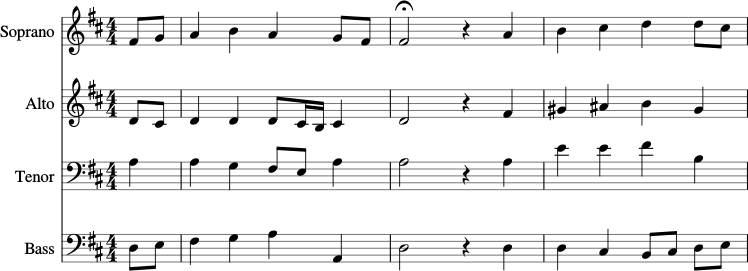
\includegraphics[width=0.8\linewidth]{Figures/bwv133-6-original-score-1.png}
    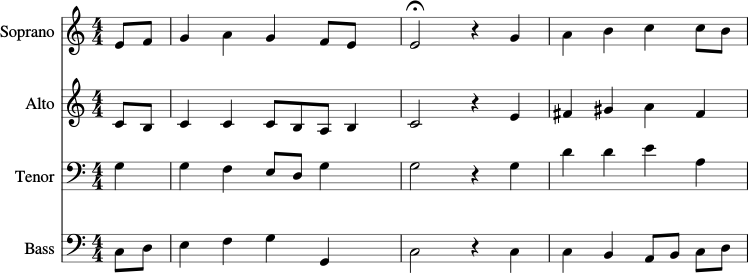
\includegraphics[width=0.8\linewidth]{Figures/bwv133-6-preproc-score-1.png}
    \caption{First 4 bars of JCB Chorale BWV 133.6 before (top) and after (bottom) preprocessing. Note
    the transposition down by a semitone to C-major as well as quantization of the
    semiquavers to quavers in Alto bar 2.}
    \label{fig:score-effects-preproc}
\end{figure}

\begin{figure}[htpb]
    \centering
        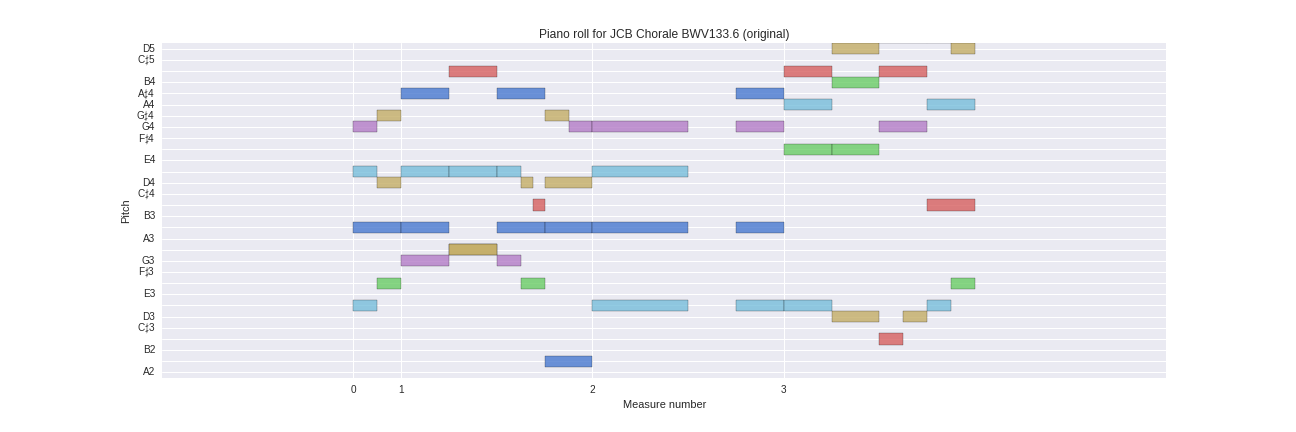
\includegraphics[width=1.0\linewidth]{Figures/bwv133-6-original-piano-roll.png}
        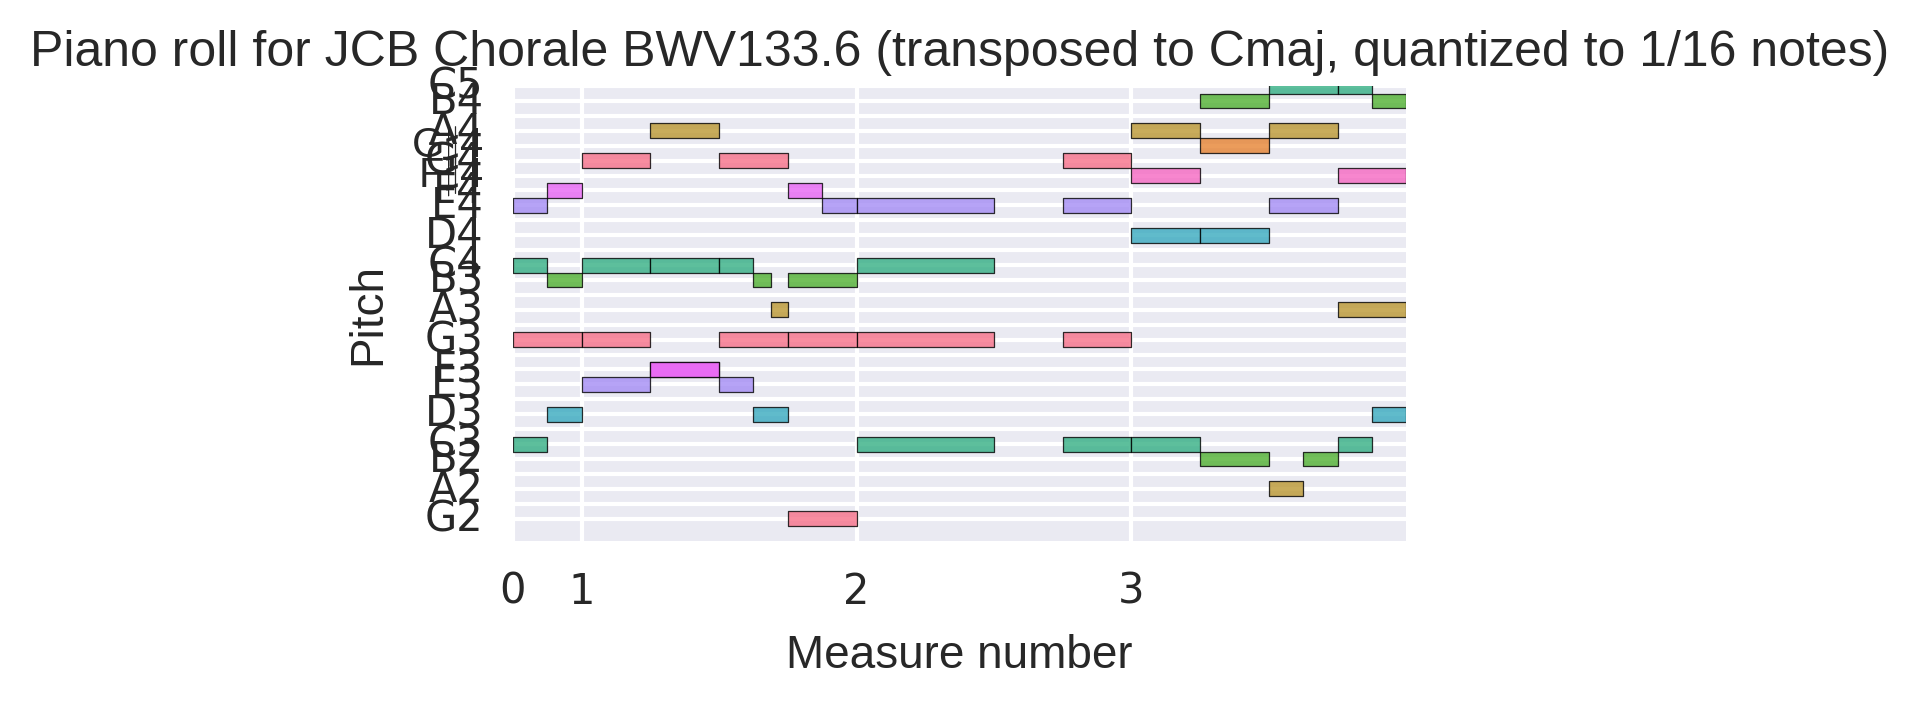
\includegraphics[width=1.0\linewidth]{Figures/bwv133-6-preproc-piano-roll.png}
    \caption{Piano roll representation of the same 4 bars from \autoref{fig:score-effects-preproc}
    before and after preprocessing.}
    \label{fig:piano-roll-effects-preproc}
\end{figure}


\subsection{Sequential encoding of musical data}

Similar to \cite{todd1989connectionist}, we represent polyphonic scores using a
localist frame-based representation where time is discretized into constant
timestep \emph{frames}. Frame based processing forces the network to learn the
relative duration of notes, a counting and timing task which
\cite{gers2002learning} demonstred LSTM is capable of. Consecutive frames are
separated by a unique delimiter (``$|||$''' in \todo{Figure of score encoded in
text}).

Each frame consists of a sequence of $\langle \text{Note}, \text{Tie} \rangle$
tuples where $\text{Note} \in \{0,1,\cdots,127\}$ represents the MIDI pitch of
a note and $\text{Tie} \in \{T,F\}$ distinguishes whether a note is tied with a
note at the same pitch from the previous frame or is articulated at the current
timestep. \todo{Order of SATB parts, bass rooting}.

The above specification describes our initial encoding. Later in our work
\todo{reference}, we found that this encoding resulted in unrealistically long
phrase lengths. Including fermatas (represented by ``(.)'' in \todo{Figure of
encoded score}, which Bach used to denote ends of phrases, solves this problem.

Finally, for each score a unique start symbol %(``ї'' in \todo{Figure})
and end symbol %(``ћ'' in \todo{Figure})
are appended to the beginning and end
repsectively. This causes the model to learn to initialize itself when given
the start symbol and allows us to determine when a composition generated by
the model has concluded.

Observe that our encoding is sparse: unarticulated notes are not encoded. It is
also variable length as anywhere from zero to four (in the case of chorales,
more for arbitrary polyphonic scores) notes. Finally, the explicit
representation of tied notes vs articulated notes solves the problem plaguing
\cite{Eck2002}\cite{eck2008learning} \cite{Liu2014} \cite{Brien2016} where
multiple articulations at the same pitch are indistinguishable from a single
note with the same duration.

Additionally, notice that our encoding avoids hand-engineered features such as
pitch representations which are psychochologically-based \cite{mozer1994neural}
or harmonically-based \cite{franklin2004recurrent}
\cite{laden1989representation}. This is intentional and is motivated by
numerous reports \cite{bengio2009learning}\cite{Bengio2011} suggesting that
that a key ingredient in deep learning's success is its ability to learn good
features from raw data.





\begin{figure}[htpb]
    \centering
    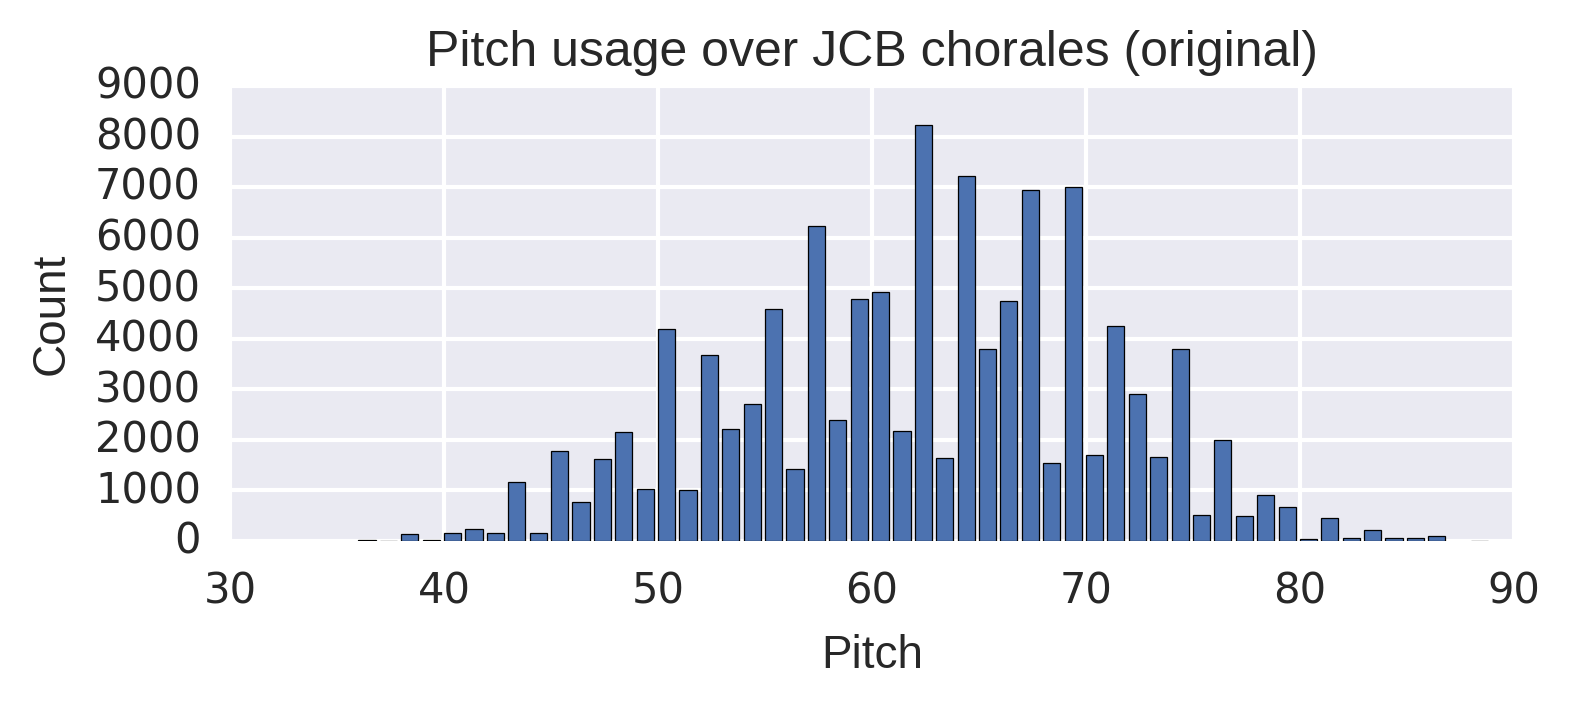
\includegraphics[width=1.0\linewidth]{Figures/pitch-usage-original.png}
    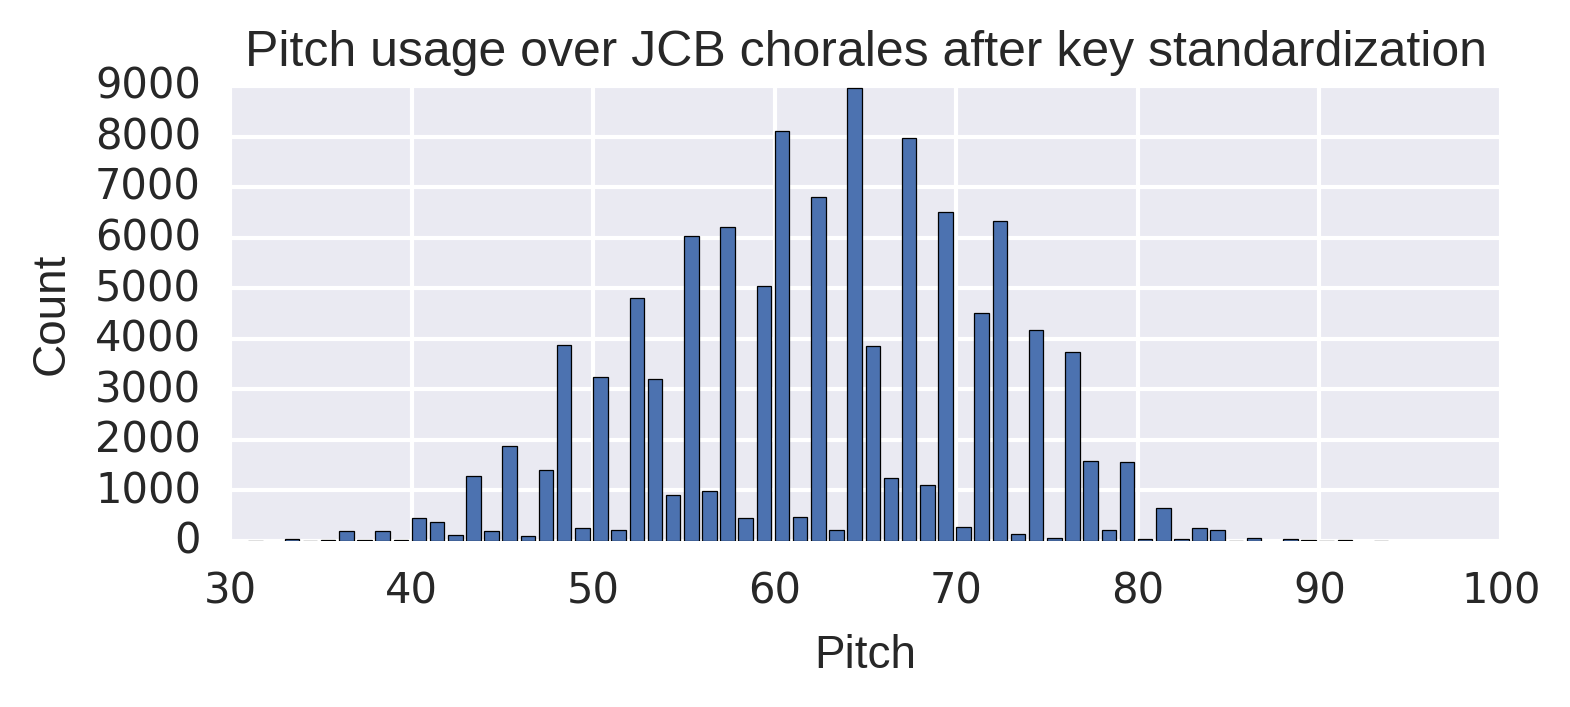
\includegraphics[width=1.0\linewidth]{Figures/pitch-usage-preproc.png}
    \caption{Pitches before and after key standardization}
    \label{fig:pitch-key-standardization}
\end{figure}

\begin{figure}
    \centering
    \begin{subfigure}[b]{0.48\textwidth}
        \centering
        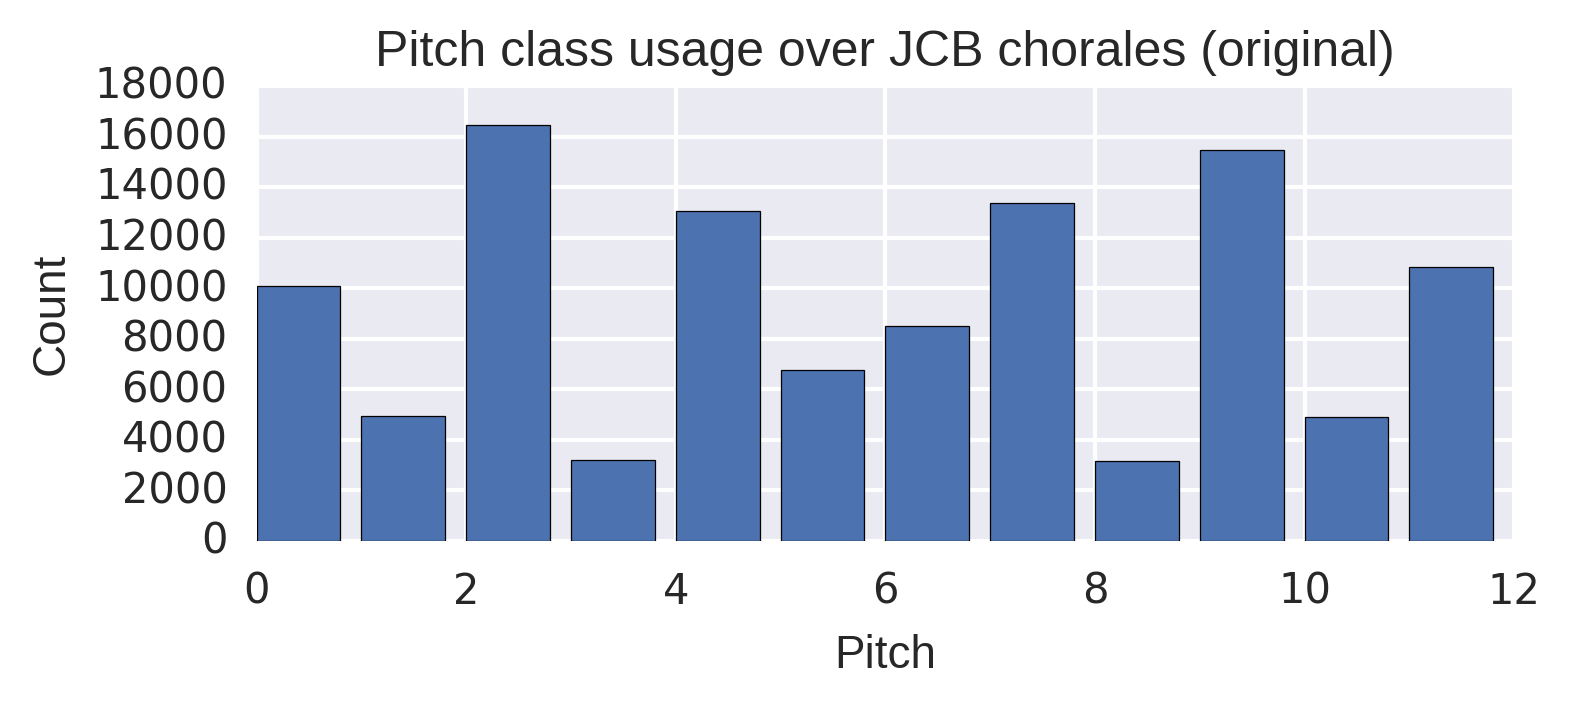
\includegraphics[width=1.0\linewidth]{Figures/pitch-class-usage-original.png}
    \end{subfigure}
    \begin{subfigure}[b]{0.48\textwidth}
        \centering
        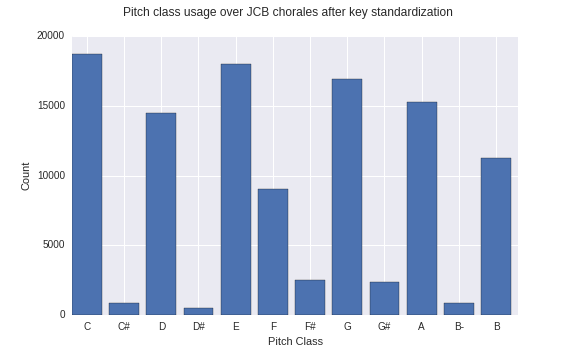
\includegraphics[width=1.0\linewidth]{Figures/pitch-class-usage-preproc.png}
    \end{subfigure}
    \caption{Pitch classes before and after key standardization}
    \label{fig:pc-key-standardization}
\end{figure}

\begin{figure}[htpb]
    \centering
    \begin{subfigure}[t]{0.48\textwidth}
        \centering
        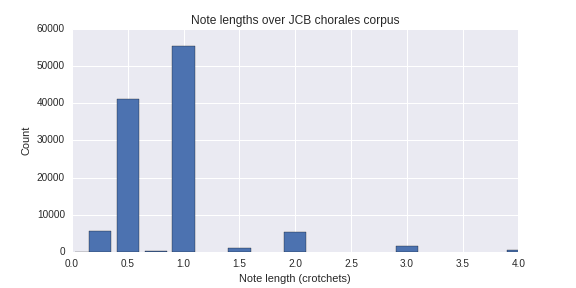
\includegraphics[width=1.0\linewidth]{Figures/note-lengths-original.png}
    \end{subfigure}
    ~
    \begin{subfigure}[t]{0.48\textwidth}
        \centering
        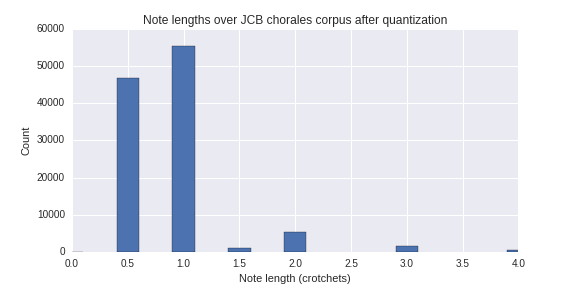
\includegraphics[width=1.0\linewidth]{Figures/note-lengths-quantized.png}
    \end{subfigure}
    \caption{Effects of time quantization on note durations}
    \label{fig:note-lengths-time-quantization}
\end{figure}

\begin{figure}[htpb]
    \centering
    \begin{subfigure}[t]{0.48\textwidth}
        \centering
        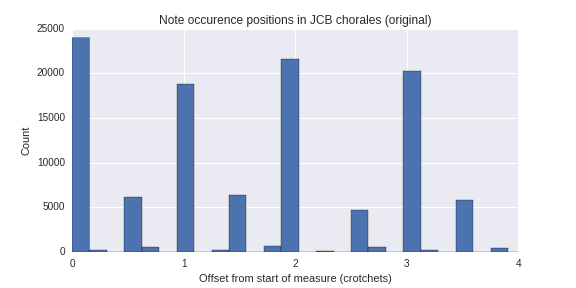
\includegraphics[width=1.0\linewidth]{Figures/meter-usage-original.png}
    \end{subfigure}
    ~
    \begin{subfigure}[t]{0.48\textwidth}
        \centering
        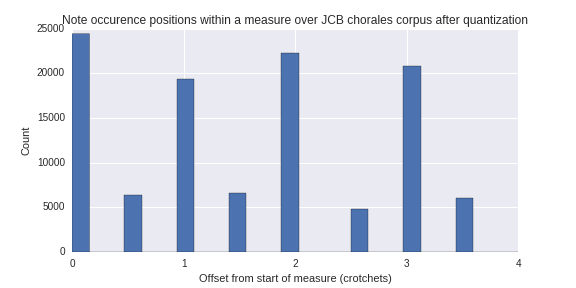
\includegraphics[width=1.0\linewidth]{Figures/meter-usage-quantized.png}
    \end{subfigure}
    \caption{Effects of time quantization on meter}
    \label{fig:meter-time-quantization}
\end{figure}



\section{Model description}

Unlike many prior models for music data, we avoid injection of
domain-specific knowledge into our models such as distinguishing between chords
versus notes \cite{hild1991harmonet}\cite{mozer1994neural} \cite{Eck2002} and
explicitly modelling of meter \cite{eck2008learning} or motifs
\cite{feulner1994melot}.

\subsubsection{Sequential processing and sampling}

Following \cite{1994neural}, we will train the model to predict a probability
distribution over all possible tokens at time $t+1$ using the token at time
$t$. We also employ \emph{teacher forcing}\cite{williams1989learning}, where
the target outputs instead of the actual outputs (i.e. most likely predicted
tokens for time $t+1$) as recurrent inputs since the model predictions may not
yet be correct during the early iterations of training.

We will train our RNNs to predict a distribution for the next character
$\x_{t+1}$ after the RNN has processed the sequence $\x_{1:t}$,
yielding a model which factorizes the sequence probability
\begin{equation}
    P(\x_{1:T}) = \prod_{t=1}^T P(\x_t | \x_{1:t-1} )
\end{equation}
Modeling this probability distribution over sequences is analogous to the
\textbf{language modeling} from speech recognition.

Note that the factorization of conditional distributions \emph{assumes a
sequential ordering in $t$}. This property is desirable as it enables sampling
from the model to generate new transcriptions by sampling from $P(\x_t |
\x_{1:t-1})$ at each timestep $t$ and using the sampled value as the next
input.

\subsection{Parameter estimation of recursive neural networks}


\subsubsection{Modeling probabilities using the Boltzmann distribution and cross-entropy error criterion}

The parameters to the model are estimated in order to minimize the error
between the network outputs and provided labels. For language modeling, the
outputs $\y_t$ should parameterize a distribution for the next character
$P(\x_{t+1} | \x_{1:t})$. Suppose each input has finite support (i.e.
$\x_t \in [1,2,\cdots,K]$). If we choose the outputs to be $K$ dimensional
(i.e. $\y_t \in \RR^K$) then the \textbf{Boltzmann distribution}
(\autoref{eq:boltzmann-dist}) can be used:

\begin{equation}
    \label{eq:boltzmann-dist}
    P(\x_{t+1} = s | \x_{1:t})
    = \frac{\exp \left(-\y_{t,s}/T\right) }{ \sum_{k=1}^{K} \left(\exp -\y_{t,k}/T\right)}
\end{equation}

$T \in \RR^+$ is a \textbf{temperature} parameter \todo{relate to sampling}.

The labels provided are the actual next characters $\x_{t+1}$. Viewing
such labels as discrete probability distributions will all mass on a single atom,
one measure of difference between predictions and \todo{justify cross-entropy}

\section{Polyphonic modeling}

\cite{Nayebi2015} reports LSTMs significantly
outperform GRUs in music applications.

\section{Technical details}

\todo{We use teacher forcing \cite{williams1989learning}}

We construct multi-layer LSTM models with \texttt{num\_layers} number of
layers, each containing \texttt{rnn\_size} hidden units. The inputs $x_t$ are
one-hot-encoded before being passed through a \texttt{wordvec}-dimensional
vector-space embedding layer, which compresses the dimensionality down from
$|V| \approx 140$ to $\texttt{wordvec}$ dimensions. Dropout layers were added
between LSTM connections in both depth and time dimensions all with dropout
probability $\texttt{dropout} \in [0,1]$.

We build our models using the \texttt{torch7} framework and
an optimized implementation of LSTMs provided by \texttt{torch-rnn} \todo{cite}.

Models were trained using RMSProp \todo{cite} with batch normalization \todo{cite}
and an initial learning rate of $2 \times 10^{-3}$ decayed by $0.5$ every $5$
epochs. The back-propogation through time gradients were clipped
at $t$ \todo{cite Mikolov} and truncated after \texttt{seq\_length} time steps.
We use a mini-batch size of $50$.

\subsection{Multi-GPU implementation}

To accelerate model training, we parallelize models across multiple GPUs. This is possible
thanks to the summation operation in noisy gradient estimators:

\begin{equation}
  \frac{1}{N} \sum_{i=1}^N \nabla L_i(\theta) \approx \frac{1}{N} \sum_{i=1}^N \nabla L_i(\theta)
\end{equation}
\todo{Real citations on noisy gradient}

In particular, training RNNs with hidden state requires sequential traversal
of the dataset. Parallelizing sequential iteration is accomplished by first segmenting
into equal length segments and then initializing parallel iterators each
pointing at a different segment. Each iterator sequentially reads data
into GPU memory.

Model parameters are broadcast out to all GPUs on each \texttt{forward} pass
and gradients are accumulated during each \texttt{backward} pass.

Research in grid LSTMs suggests that we can go deeper by introducing
gates along the depth dimension to help permit information flow \todo{cite gird LSTMs}.

\section{Results}

Compare with \cite{Allan2005} and \cite{Brien2016}.

\printbibliography

\end{document}

\documentclass[dissertation.tex]{subfiles}
\begin{document}

\chapter{Large-scale subjective evaluation}

\cite{pearce2001towards} addresses difficulty in quantitative evaluation,
suggesting the use of a learned critic in a manner similar to GANs
\cite{goodfellow2014generative}. In a later report,
\cite{pearce2002motivations} attribute difficulty in evaluation due to lack
aim: algorithmic composition, design of compositional tools, and computational
modelling of musical styles or music cognition all have different motivations
and should thus be evaluated differently.

Following advice of \cite{pearce2002motivations}, we identify our key
motivation as algorithmic composition: generation of novel compositions.
To evaluate our success, we employ a subjective evaluation method.

\cite{ariza2009} criticizes a musical Turing test as providing little data about
how to improve the system, suggesting that listener studies using music experts
may be more insightful.



The frontend utilizes React and Redux, allowing us to collect fine-grained user
action data. Azure App Service is used to host an Express web-service which
randomizes experimental questions and collects responses. The data is stored to
Azure Data Storage and processed in batch MapReduce using Azure HDInsight.

We ask users to rate themselves on their musical skills (0-10) and present the
user with five questions. Each questions asks the user to listen to two
samples, one generated and one original Bach, and tasks the user to select the
original. In addition to the question response, we collect data on the time
spent on a questions and number of times each sample is played.

\section{Results}

\begin{figure}[htpb]
  \centering
  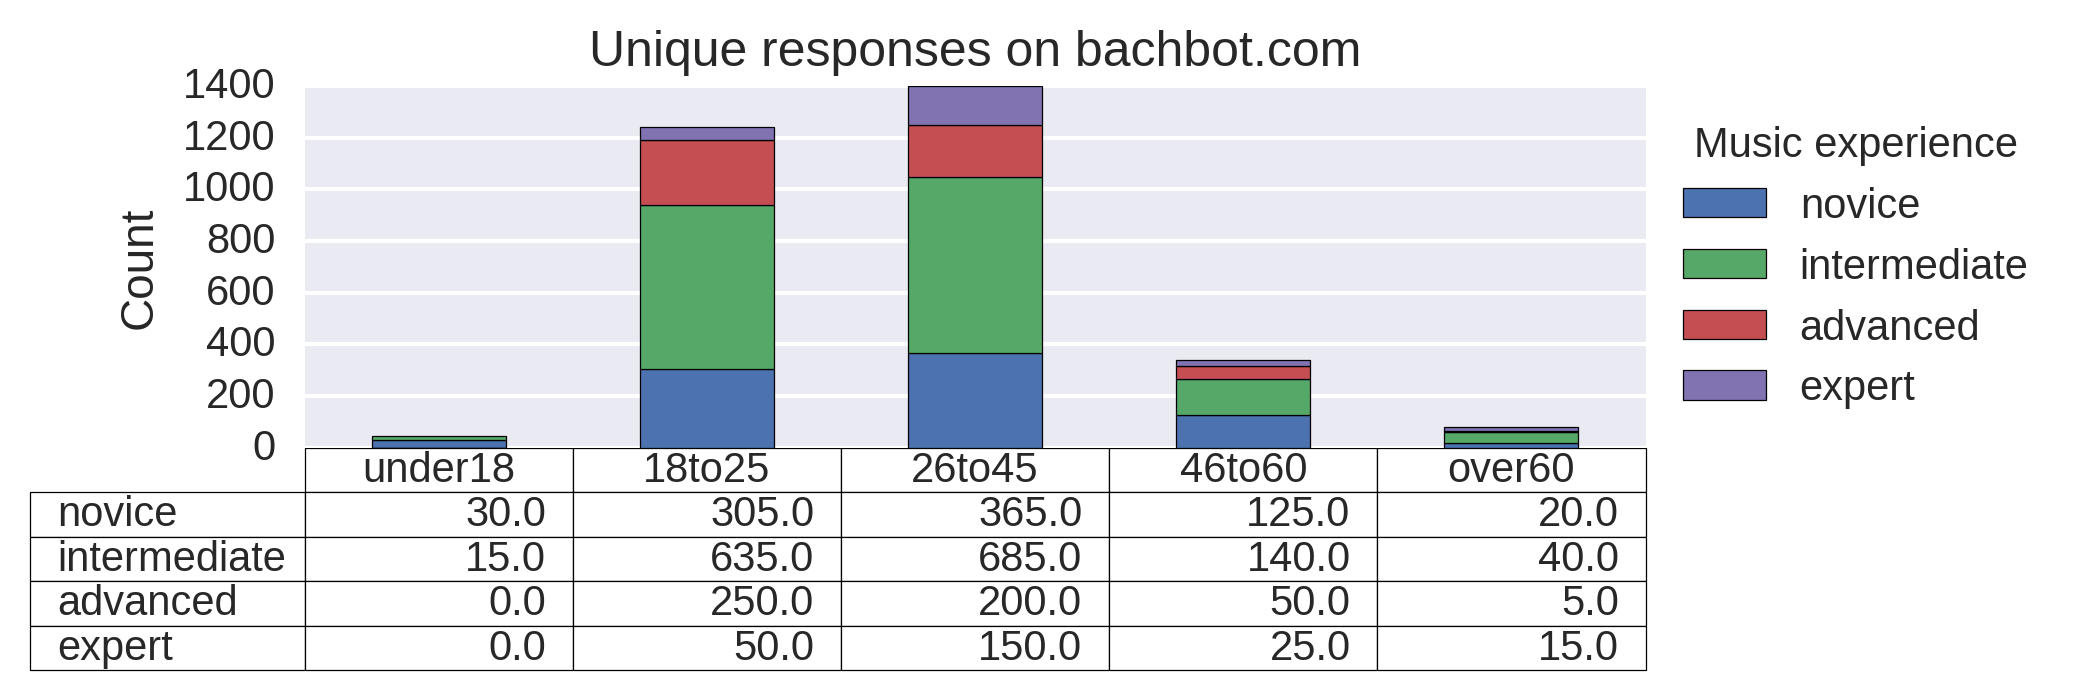
\includegraphics[width=1.0\linewidth]{Figures/responses-ageGroup-musicExperience.png}
  \caption{Demographic breakdown of participants}
  \label{fig:responses-ageGroup-musicExperience}
\end{figure}

\todo{\autoref{fig:responses-mask} suggests performance is weakest on
  harmonizations. Unsurprising because we only do 1-best and don't account
  for future. Bidirectional LSTM or N-best lattice search (reference marcin)
  would do better}
\begin{figure}[htpb]
  \centering
  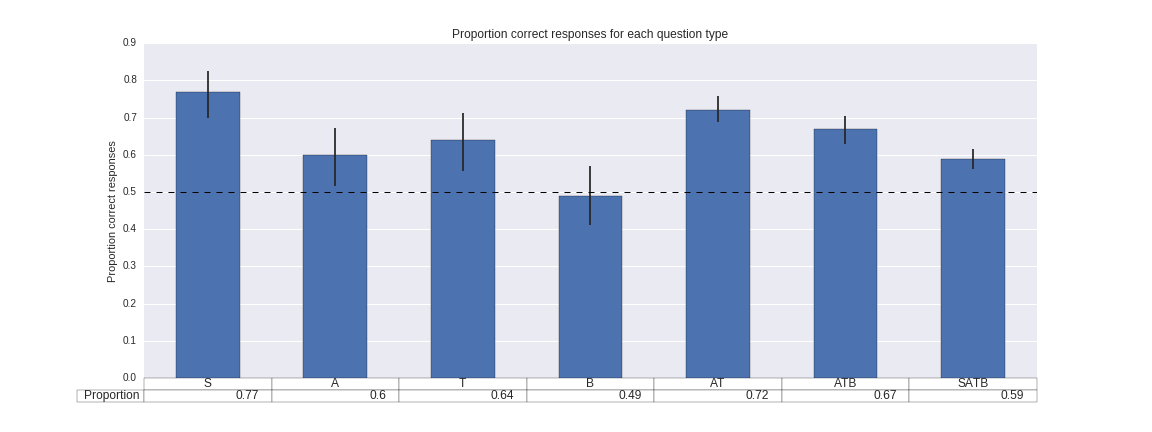
\includegraphics[width=1.0\linewidth]{Figures/responses-mask.png}
  \caption{Figures/responses-Mask}
  \label{fig:responses-mask}
\end{figure}

\begin{figure}[htpb]
  \centering
  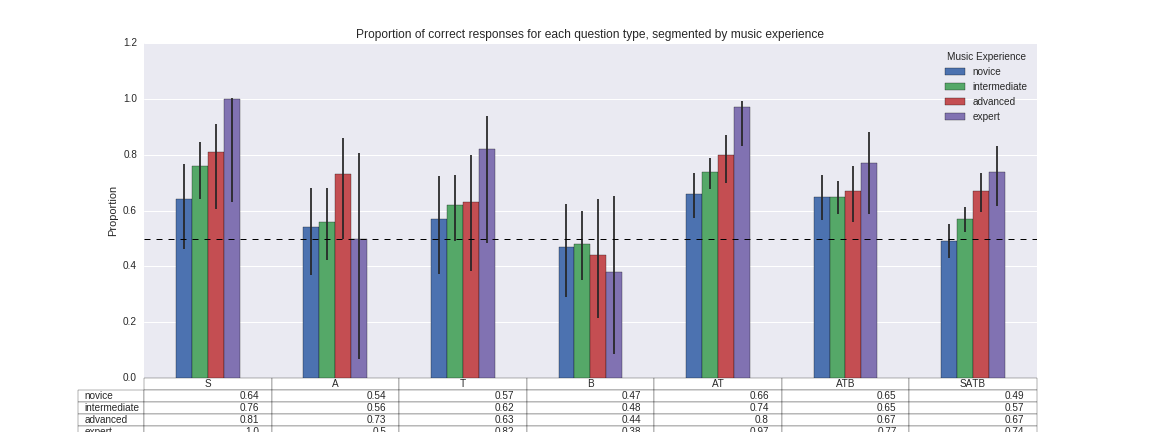
\includegraphics[width=1.0\linewidth]{Figures/responses-mask-musicExperience.png}
  \caption{Figures/responses-mask-MusicExperience}
  \label{fig:responses-mask-musicExperience}
\end{figure}

\begin{figure}[htpb]
  \centering
  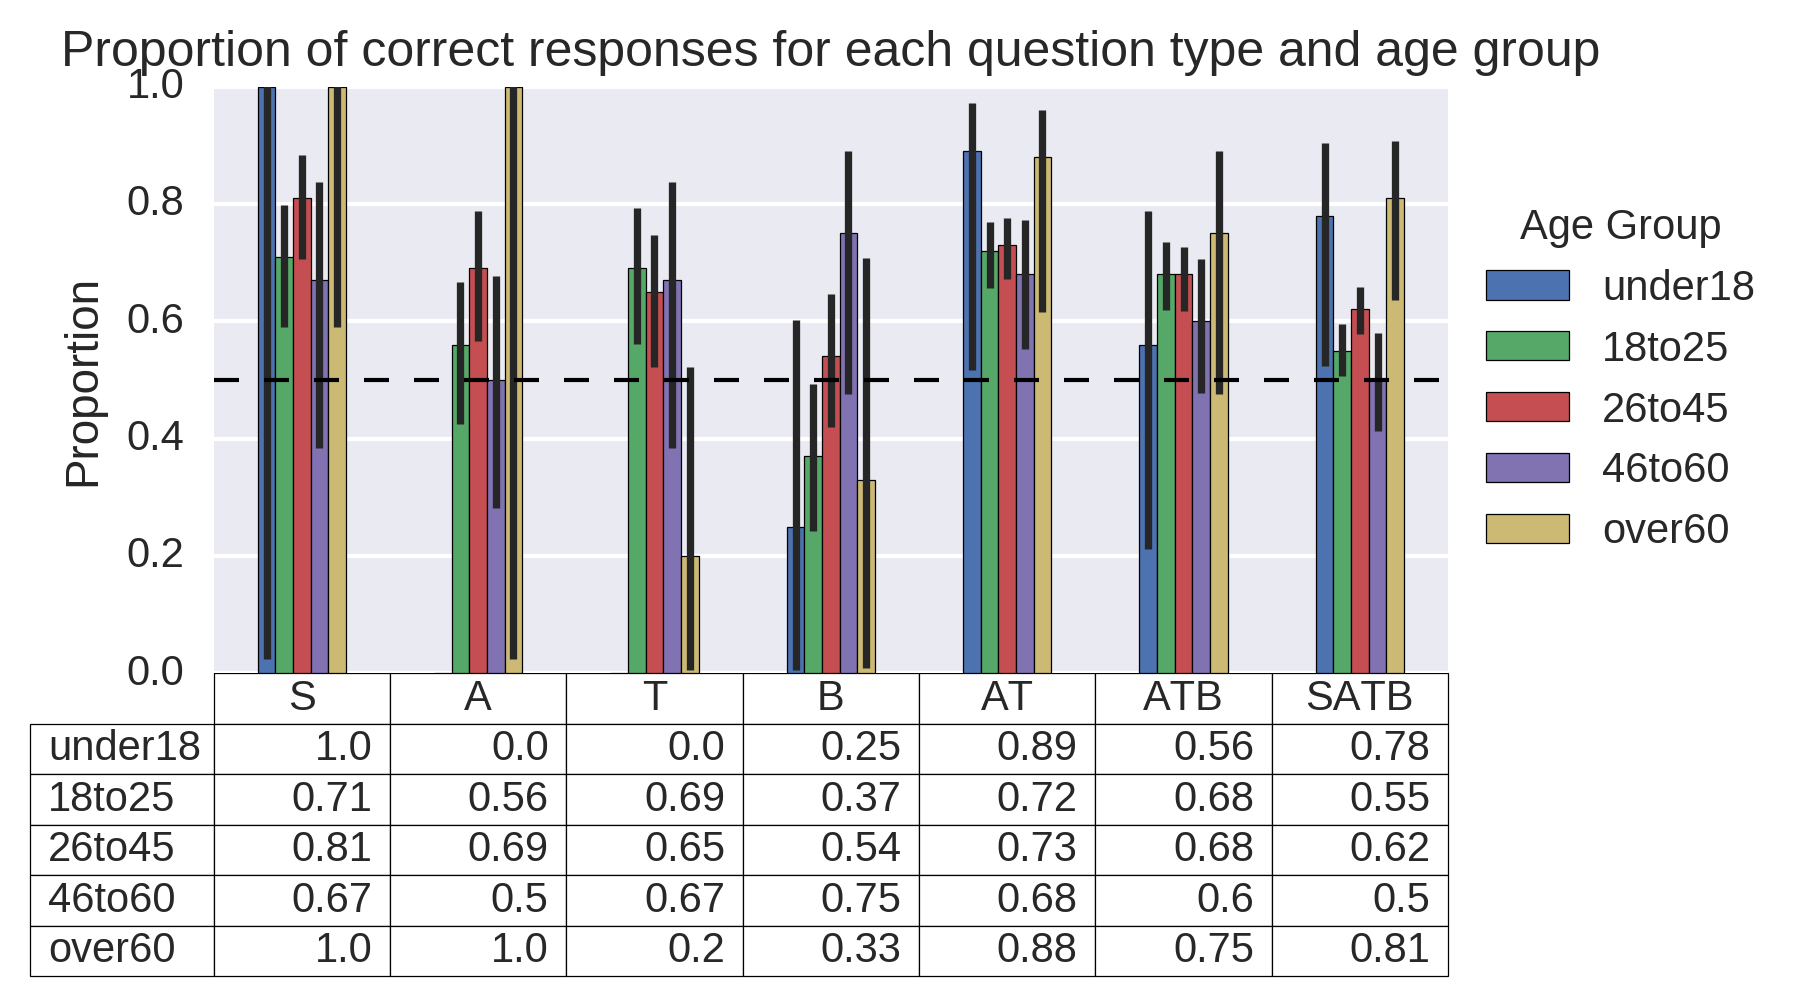
\includegraphics[width=1.0\linewidth]{Figures/responses-mask-agegroup.png}
  \caption{Figures/responses-mask-Agegroup}
  \label{fig:responses-mask-agegroup}
\end{figure}

\begin{figure}[htpb]
  \centering
  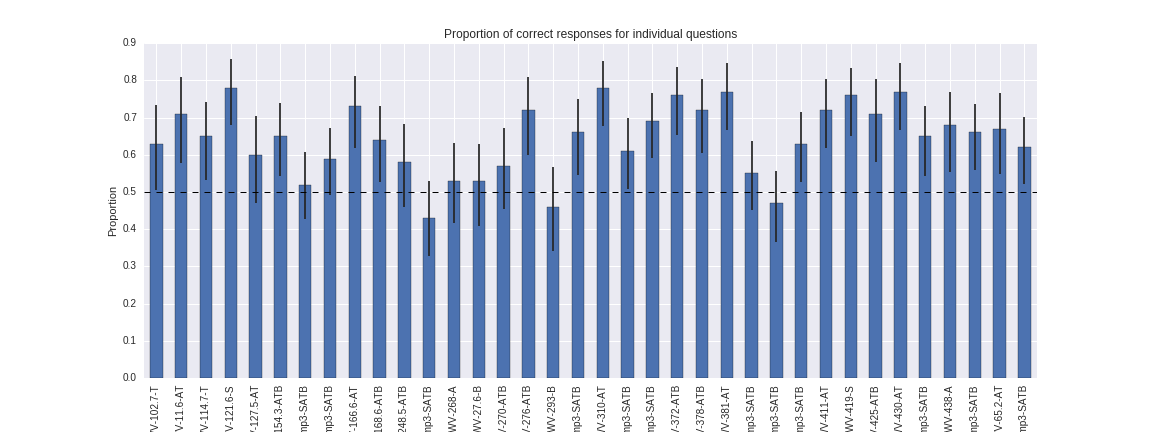
\includegraphics[width=1.0\linewidth]{Figures/responses-name.png}
  \caption{Proportion of correct responses broken down by individual questions.}
  \label{fig:responses-name}
\end{figure}

\todo{Analyze why bad questions in \autoref{fig:responses-name} are happening}

\section{User feedback}

The modulations and part writing were the giveaway for me (and once or twice the phrasing)

Got 5/5. The trick is to listen for the unnatural pauses at regular intervals.

Cool project, I scored 100\% so I'm quite pleased with myself ;o) I do
play an instrument although I'm not classical trained. If I had an
inkling to why I could choose the background phrasing of the Bach
pieces is far more elegant than the computer generated pieces.

@samim @feynmanliang really impressive! If I didn't know about counterpoint that quiz would've stumped me



\printbibliography

\end{document}


\appendix
\singlespacing

\bibliographystyle{unsrt}
\bibliography{refs}

\printindex

\end{document}
